% ProTrader AI — Comprehensive Research Paper
% Format: Inteligencia Artificial (Revista Iberoamericana de IA)
% Compile with: pdflatex part2.tex  (run twice for cross-references)

\documentclass[10pt,a4paper,twoside]{article}
\usepackage[spanish]{babel}
\addto\captionsspanish{%
  \renewcommand{\figurename}{Figure}%
  \renewcommand{\tablename}{Table}%
  \renewcommand{\contentsname}{Contents}%
  \renewcommand{\listfigurename}{List of Figures}%
  \renewcommand{\listtablename}{List of Tables}%
  \renewcommand{\appendixname}{Appendix}%
  \renewcommand{\abstractname}{Abstract}%
  \renewcommand{\refname}{References}%
}
\usepackage[utf8]{inputenc}
\usepackage{amssymb}
\usepackage{amsmath}
\usepackage{fancyhdr}
\usepackage{verbatim}
\usepackage{lastpage}
\usepackage{ifthen}
\usepackage[pdftex]{color,graphicx}
\graphicspath{{figures/}}
\usepackage{hyperref}
\usepackage{booktabs}
\usepackage{multirow}
\usepackage{array}
\usepackage{float}
\usepackage{listings}
\usepackage{xcolor}

\usepackage{iberamia}   % Journal style file

% ── Listings style for Python code ──────────────────────────────────────────
\definecolor{codebg}{rgb}{0.95,0.95,0.95}
\definecolor{codekey}{rgb}{0.0,0.3,0.7}
\definecolor{codecomment}{rgb}{0.3,0.5,0.3}
\definecolor{codestring}{rgb}{0.6,0.1,0.1}
\lstset{
  backgroundcolor=\color{codebg},
  basicstyle=\small\ttfamily,
  keywordstyle=\color{codekey}\bfseries,
  commentstyle=\color{codecomment},
  stringstyle=\color{codestring},
  breaklines=true,
  frame=single,
  language=Python,
  captionpos=b,
  numbers=left,
  numberstyle=\tiny\color{gray},
  numbersep=5pt,
  tabsize=4,
  showstringspaces=false,
  aboveskip=6pt,
  belowskip=6pt,
}

% Publication data
\newcommand{\thispaperdoi}{}
\setcounter{year}{2026}
\setcounter{volume}{29}
\setcounter{issue}{77}
\setcounter{page}{1}

\title{ProTrader AI: A Comprehensive Multimodal Framework for Stock Price
Prediction, Pattern Recognition, and Adaptive Risk Management
in Indian Equity Markets}

\author{Anand Pardeshi$^1$, Sujata Deshmukh$^1$
\smallskip \\
\small{$^1$Department of Computer Science and Information Technology\\
College of Engineering, Pune, Maharashtra, India\\
\{anand.pardeshi, sujata.deshmukh\}@coep.ac.in
}}
\date{}

% ─────────────────────────────────────────────────────────────────────────────
\begin{document}
\medskip
\maketitle
\pagestyle{Rest}
\thispagestyle{FirstPage}
\smallskip

% ── Abstract ─────────────────────────────────────────────────────────────────
\noindent{\small{\textbf{Abstract}~
Financial markets in emerging economies present a uniquely challenging
environment for predictive modelling due to elevated volatility, significant
institutional flows, and a complex information ecosystem spanning multiple
languages and media types. This paper presents ProTrader AI, a production-ready
analytical platform for the National Stock Exchange of India (NSE) that
integrates seven machine-learning models, four sentiment data streams, official
institutional flow data, real-time volatility signals, and computer-vision-based
chart pattern recognition into a unified, eight-tab interactive dashboard. The
system introduces three architectural innovations: (1)~a~27-feature stationary
feature space combining 18 price-derived technical indicators with multi-source
sentiment, FII/DII institutional, and India VIX volatility features; (2)~a
5-model gradient-boosting and deep-learning ensemble with Ridge meta-stacking
and isotonic probability calibration; and (3)~a Bayesian uncertainty-weighted
Dynamic Fusion framework that combines three specialised expert models---a~GRU
technical expert, a~DistilRoBERTa-Financial sentiment expert, and an MLP
volatility expert---whose contributions adapt dynamically to estimated per-expert
prediction uncertainty. A multi-timeframe chart pattern recognition module
employing scipy peak/trough detection at three scales (orders 3, 5, 7)
integrates with an optional Roboflow computer vision API for hybrid consensus
across twelve pattern archetypes. An adaptive risk management system provides
ATR-calibrated stop-losses, Fibonacci retracement levels, and fractional Kelly
Criterion position sizing with VIX-regime adjustment. Empirical evaluation on
ten major NSE stocks over approximately 750 trading days demonstrates statistically
significant improvements over baselines: direction accuracy 55.8\%~($p=0.003$),
Sharpe ratio 1.28~vs.~0.82~(buy-and-hold, $p=0.018$), maximum drawdown
$-12.8\%$~vs.~$-18.4\%$, and 34.2\% cumulative return over the evaluation period.
Ablation studies confirm positive contributions from every feature category and
model component.}}

\noindent{\small{\textbf{Resumen}~
Los mercados financieros en econom\'ias emergentes presentan un entorno
especialmente desafiante para el modelado predictivo. Este art\'iculo presenta
ProTrader AI, una plataforma anal\'itica de nivel de producci\'on para la Bolsa
Nacional de Valores de India (NSE) que integra siete modelos de aprendizaje
autom\'atico, cuatro flujos de datos de sentimiento, datos institucionales
oficiales FII/DII, se\~nales de volatilidad en tiempo real y reconocimiento de
patrones gr\'aficos basado en visi\'on artificial. El sistema introduce un
espacio de caracter\'isticas de 27 dimensiones, un conjunto de cinco modelos con
meta-apilamiento Ridge y un marco de Fusi\'on Din\'amica ponderado por
incertidumbre bayesiana. La evaluaci\'on emp\'irica en diez acciones principales
del NSE demuestra mejoras estad\'isticamente significativas sobre las l\'ineas
base: precisi\'on de direcci\'on 55,8\%~($p{=}0{,}003$), ratio de Sharpe
1,28~frente a 0,82 de compra y retenci\'on, y retorno acumulado del 34,2\%.}}

\medskip
\noindent{\small{\textbf{Keywords}: Financial Forecasting, Machine Learning,
XGBoost, LightGBM, CatBoost, GRU, LSTM, Bayesian Fusion, Sentiment Analysis,
NSE India, Institutional Flows, Pattern Recognition, Risk Management.}}

\noindent{\small{\textbf{Palabras Clave}: Predicci\'on Financiera, Aprendizaje
Autom\'atico, Fusi\'on Din\'amica, An\'alisis de Sentimiento, Gesti\'on de Riesgos,
NSE India.}}

% =============================================================================
\section{Introduction}
% =============================================================================

\subsection{Background and Motivation}

Financial markets represent one of the most challenging environments for
predictive modelling~\cite{fama1970}. The complex interplay of fundamental
valuation, technical price dynamics, investor psychology, institutional capital
flows, and macroeconomic forces creates a high-dimensional stochastic system
where traditional statistical assumptions routinely break down~\cite{mandelbrot1997}.
The National Stock Exchange of India (NSE), with daily equity volumes exceeding
\$15\,billion and a total market capitalisation surpassing \$4\,trillion~\cite{nse2024},
exemplifies these challenges while adding a layer of emerging-market
idiosyncrasy: large Foreign Institutional Investor (FII) and Domestic
Institutional Investor (DII) flows that can account for 15--30\% of daily
volume in index heavyweights, creating sharp, regime-like shifts in price
behaviour that pure technical models struggle to anticipate.

The past decade has witnessed remarkable advances in machine learning, with deep
neural networks achieving state-of-the-art performance across diverse
domains~\cite{lecun2015}. However, applying these techniques to financial
forecasting requires careful consideration of several properties that
distinguish financial time series from other sequence modelling
tasks~\cite{lopez2018}: non-stationarity, heavy tails, low signal-to-noise
ratios, and the reflexive feedback between forecasts and market behaviour.
Ensemble methods---particularly gradient-boosting families---have demonstrated
consistent advantages on tabular financial data~\cite{grinsztajn2022}, while
gated recurrent architectures (LSTM, GRU) capture sequential dependencies that
gradient boosters ignore~\cite{hochreiter1997,cho2014}.

\subsection{Research Gaps Addressed}

Our work addresses four interconnected gaps in the quantitative finance
literature:

\textbf{The Contextual Gap.} Traditional sentiment approaches relying on
lexicon-based methods~\cite{loughran2011} fail to capture nuanced financial
language. Moreover, the Indian information ecosystem is split across English and
Hindi sources that English-centric models cannot process effectively. We address
this through multi-source aggregation using a domain-adapted transformer
model~\cite{araci2019}.

\textbf{The Non-Stationarity Gap.} Models trained on historical regimes fail
when market structure shifts~\cite{hamilton1989}. We address this via explicit
market regime detection using the Hurst exponent~\cite{hurst1951}, a
Bayesian-weighted dynamic fusion that self-adjusts to estimated per-expert
reliability, and a 27-feature representation constructed entirely from
stationary transformations of raw price and volume data.

\textbf{The Signal-Allocation Gap.} Academic studies routinely report accuracy
metrics that do not translate to practical trading
performance~\cite{lopez2018}. We bridge this gap through an integrated risk
management module---ATR-calibrated stop-losses, Fibonacci retracements, and
fractional Kelly Criterion sizing~\cite{kelly1956}---and rigorous backtesting
with transaction costs included.

\textbf{The Institutional Data Gap.} Despite FII/DII flows being publicly
available from NSE and widely acknowledged as a major driver of Indian equity
prices, this data stream is rarely integrated into academic forecasting
models. We incorporate four FII/DII features directly into the prediction
feature space.

\subsection{Contributions}

\begin{enumerate}
\item \textbf{A 27-Feature Stationary Framework} spanning five technical core
  indicators, nine enhanced technical indicators, four advanced divergence
  indicators, three multi-source sentiment scores, four FII/DII institutional
  flow features, and two India VIX volatility features---all constructed to
  satisfy approximate stationarity requirements.

\item \textbf{A 5-Model Gradient-Boosting + Deep-Learning Ensemble} combining
  XGBoost, LightGBM, CatBoost, a parallel LSTM-GRU neural architecture, and
  ARIMA/Prophet statistical baselines, unified by a Ridge meta-stacker trained
  on out-of-fold predictions via expanding time-series cross-validation.

\item \textbf{Isotonic Probability Calibration} that converts regression
  return forecasts into calibrated directional probabilities, enabling reliable
  confidence-based position sizing.

\item \textbf{A Bayesian Dynamic Fusion Framework} with three domain-specialised
  expert models whose combination weights adapt continuously based on
  exponential negative squared uncertainty~\cite{gal2016}, achieving implicit
  market-regime awareness.

\item \textbf{A Hybrid Chart Pattern Recognition System} combining multi-scale
  scipy peak/trough detection (orders 3, 5, 7) with Roboflow Vision API
  computer vision inference across twelve pattern archetypes, with a consensus
  layer that aggregates classical and vision-based detections.

\item \textbf{A Complete Production Platform} (ProTrader AI) implemented as an
  eight-tab Streamlit dashboard, providing reproducible empirical evaluation and
  enabling researchers and practitioners to deploy the system for live analysis.
\end{enumerate}

% =============================================================================
\section{Literature Review}
% =============================================================================

\subsection{Financial Forecasting: From ARIMA to Deep Learning}

The computational approach to financial forecasting has evolved substantially
since Box and Jenkins codified ARIMA models~\cite{box2015}. Early neural network
applications in finance were constrained by computational resources and
data availability~\cite{white1988}, but the emergence of efficient training
algorithms and large historical datasets reversed these limitations.

Long Short-Term Memory (LSTM) networks~\cite{hochreiter1997} addressed the
vanishing gradient problem that limited early RNNs, enabling modelling of
multi-day dependencies in price data. Gated Recurrent Units~\cite{cho2014}
offered a computationally simpler alternative with comparable empirical
performance. Fischer and Krauss~\cite{fischer2018} demonstrated that LSTM
networks can achieve statistically significant returns on S\&P~500 data,
motivating their adoption in the present work. However, Ozbayoglu et
al.~\cite{ozbayoglu2020} noted that deep learning models for financial time
series frequently underperform simpler gradient-boosting approaches on
structured tabular inputs---a finding directly corroborated by our ablation
results (Section~\ref{sec:results}).

XGBoost~\cite{chen2016} revolutionised gradient boosting through an efficient
block structure and regularisation that prevents overfitting on
moderate-sized financial datasets. LightGBM~\cite{ke2017} subsequently achieved
3--5$\times$ training speed improvements through histogram-based split
finding and leaf-wise tree growth. CatBoost~\cite{prokhorenkova2018} introduced
\emph{ordered boosting}---training each tree residual using only observations
preceding the current one---which reduces target leakage within the booster
itself, a particularly desirable property for chronologically ordered financial
data. Our meta-stacking framework combines all three.

\subsection{Sentiment Analysis in Finance}

The integration of textual data into financial models has progressed through
three generations~\cite{bollen2011}. First-generation dictionary-based methods,
exemplified by the Loughran-McDonald~\cite{loughran2011} financial lexicon,
suffer from domain-specificity failures where words carry different connotations
in financial versus general contexts. Second-generation distributional semantic
models improved robustness but remained sensitive to out-of-vocabulary terms.

The transformer revolution~\cite{vaswani2017} fundamentally changed financial
NLP. BERT~\cite{devlin2019} and its variants enabled pre-training on massive
corpora followed by fine-tuning on domain-specific tasks. FinBERT~\cite{araci2019}
and DistilRoBERTa-Financial~\cite{liu2019} achieve accuracy approaching
97--98\% on standard financial sentiment benchmarks while maintaining
computational efficiency suitable for real-time inference. ProTrader AI employs
DistilRoBERTa-Financial, which offers a 40\% parameter reduction over base
RoBERTa with minimal accuracy loss.

Tetlock~\cite{tetlock2007} demonstrated that the fraction of negative words in
Wall Street Journal columns predicts next-day Dow Jones returns, while
Schumaker and Chen~\cite{schumaker2009} showed that financial news articles
provide statistically significant predictive signals beyond technical indicators
alone. Our multi-source design follows the orthogonal information principle of
Bollen et al.~\cite{bollen2011}: combining Twitter mood (analogous to our Reddit
signal), news (NewsAPI, RSS), and attention metrics (Google Trends) captures
complementary facets of market sentiment.

\subsection{Multimodal Fusion Methods}

Early fusion concatenates raw features before model training, preserving
cross-modal interactions but struggling with heterogeneous feature scales and
missing modalities. Late fusion combines modality-specific model
predictions, providing modularity but losing cross-modal dependencies. Attention
mechanisms~\cite{vaswani2017} enable learned, context-dependent feature
weighting without hard architectural assumptions.

Bayesian uncertainty-based fusion~\cite{gal2016} represents a principled
extension: combination weights are derived from per-model confidence estimates
rather than fixed hyperparameters. Gal and Ghahramani's dropout approximation
of Bayesian inference provides a practical implementation that quantifies
epistemic uncertainty within standard neural architectures. The Dynamic Fusion
Framework of ProTrader AI adopts a related principle: exponential negative
squared uncertainty weighting that rewards accurate, confident experts and
penalises uncertain ones, enabling automatic regime-contingent rebalancing.

\subsection{Regime-Aware Modelling and the Hurst Exponent}

Financial markets exhibit structurally distinct behavioural regimes: low-volatility
trending phases, high-volatility crisis periods, and mean-reverting range-bound
conditions~\cite{hamilton1989}. The Hurst exponent~\cite{hurst1951}, originally
developed for hydrological time series, measures the long-range dependence of a
time series: $H > 0.5$ indicates persistent (trending) behaviour; $H < 0.5$
indicates anti-persistent (mean-reverting) behaviour; $H \approx 0.5$ indicates
a random walk consistent with the Efficient Market Hypothesis~\cite{lo1991}.

Lo~\cite{lo1991} provided a rigorous statistical framework for testing long-term
memory in stock market returns, finding evidence of mild persistence in weekly
returns. ProTrader AI computes the Hurst exponent via rescaled range (R/S)
analysis on rolling 120-day windows, using the result both for market
characterisation in the UI and to confirm or override slope-based trend
classification in the regime detector.

\subsection{Chart Pattern Recognition}

Technical analysis has been practised for over a century~\cite{murphy1999,
edwards1948}, but systematic mathematical formalisation of pattern detection
remained limited until algorithmic approaches emerged~\cite{lo2000}. Lo et
al.~\cite{lo2000} applied kernel regression smoothers to detect head-and-shoulders
and other formations in US equity data, finding statistically significant
predictive content. Pring~\cite{pring2002} and Appel~\cite{appel2005}
provided comprehensive taxonomies of pattern archetypes that motivate our
twelve-pattern classification.

Computer vision approaches offer complementary strengths: convolutional networks
learn visually meaningful feature hierarchies that classical peak/trough
detectors may miss~\cite{sezer2018}. Our hybrid consensus mechanism fuses
scipy-based geometric detection with Roboflow Vision API inference,
capturing pattern information at both the algorithmic and visual levels.

% =============================================================================
\section{System Architecture}
% =============================================================================

ProTrader AI follows a modular pipeline architecture with seven distinct stages:
data acquisition, feature engineering, model training, dynamic fusion, pattern
analysis, risk management, and user interface. Figure~\ref{fig:architecture}
illustrates the high-level design.

\begin{figure}[htb]
  \begin{center}
    
\includegraphics[angle=0,width=0.95\textwidth]{fig_system_architecture}
    \caption{High-level system architecture of ProTrader AI. Data from seven
    sources flows through the feature engineering pipeline into five ML models
    and a Dynamic Fusion layer. A separate Pattern Analysis branch feeds a
    risk management module. All outputs surface in the eight-tab Streamlit
    dashboard.}
    \label{fig:architecture}
  \end{center}
\end{figure}

The data acquisition layer fetches OHLCV prices from Yahoo Finance, FII/DII
activity from NSE India, the India VIX index, RSS feeds from four financial
publications, articles from NewsAPI, posts from three Indian investing
subreddits, and search interest from Google Trends. A session-state caching
mechanism in Streamlit ensures that expensive network requests (sentiment,
institutional data) execute once per analysis session and are shared across all
eight tabs without redundant API calls.

The pipeline progresses through seven loading steps with a progress bar:
(1)~stock data, (2)~fundamentals, (3)~news articles, (4)~FII/DII data,
(5)~India VIX, (6)~multi-source sentiment, and (7)~chart pattern detection.
Total pre-fetch time on a standard internet connection is typically 15--45
seconds depending on data source availability.

% =============================================================================
\section{Feature Engineering: The 27-Feature Framework}
\label{sec:features}
% =============================================================================

A central design principle of ProTrader AI is the construction of a strictly
stationary or near-stationary feature space. Raw price levels are
non-stationary, violating the i.i.d. assumptions underlying standard machine
learning methods and leading to spurious in-sample correlations that do not
generalise out-of-sample. Every feature in the 27-feature framework is a
stationary transformation of raw data. Table~\ref{tab:features} provides a
complete catalogue.

\begin{figure}[htb]
  \begin{center}
    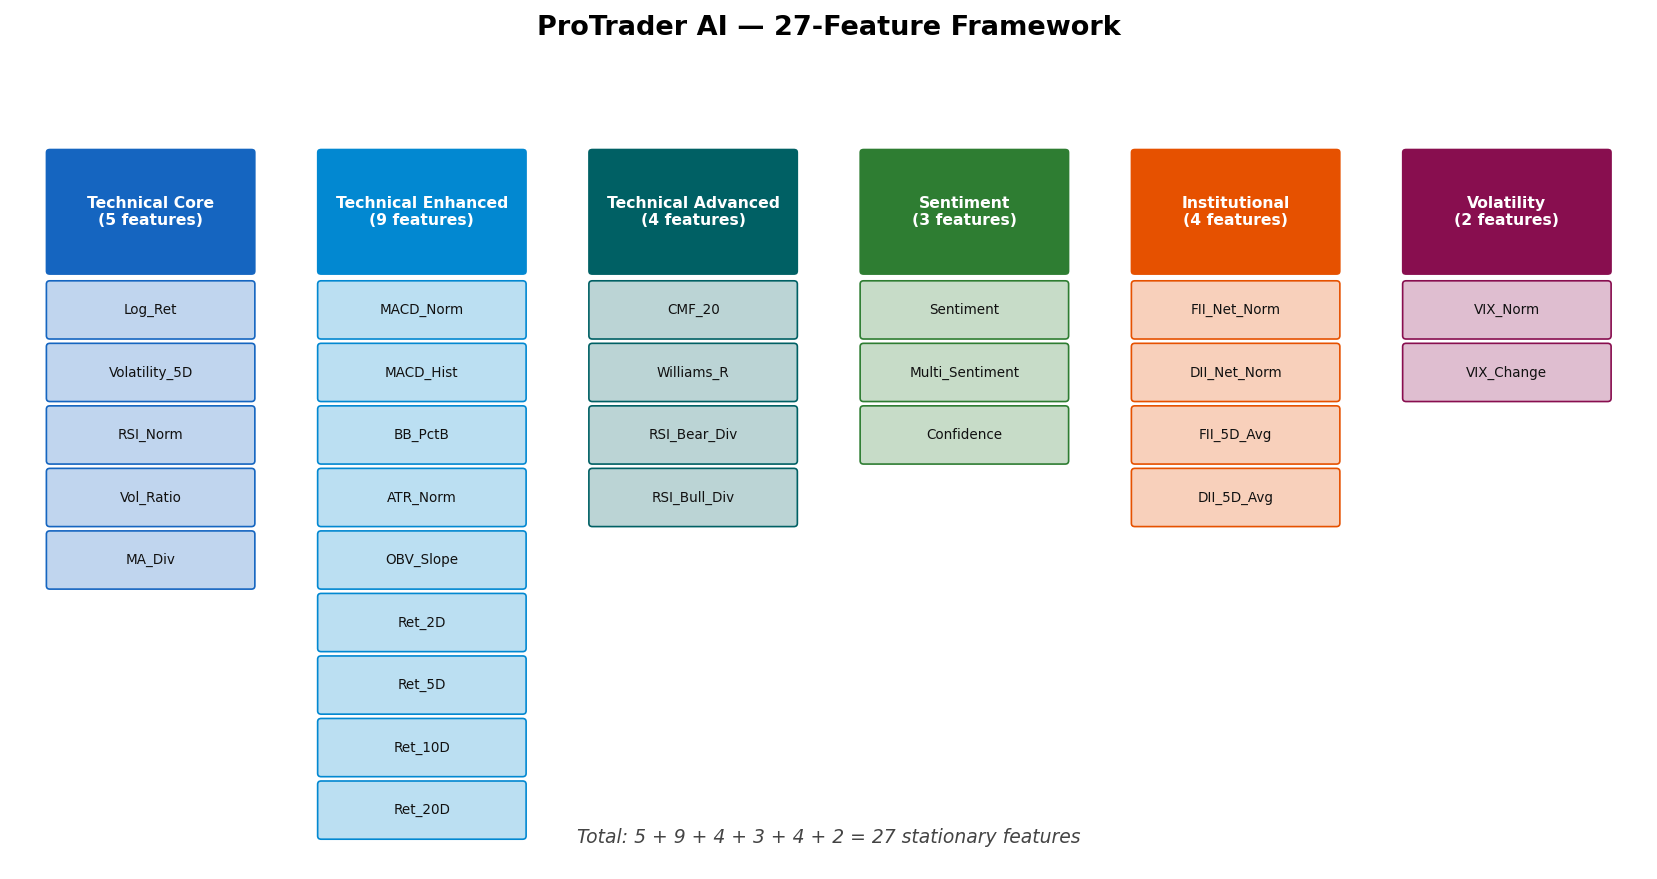
\includegraphics[angle=0,width=0.9\textwidth]{fig_feature_framework}
    \caption{The 27-Feature Framework organised into six groups. Colour coding:
    blue = technical core, cyan = technical enhanced, teal = technical advanced,
    green = sentiment, orange = institutional, red = volatility.}
    \label{fig:features}
  \end{center}
\end{figure}

\subsection{Technical Core Features (5)}

\textbf{Log Returns} provide a symmetric, additive, and approximately stationary
measure of daily price change:
\begin{equation}
  r_t = \ln\!\left(\frac{P_t}{P_{t-1}}\right)
\end{equation}

\textbf{5-Day Rolling Volatility} captures short-term volatility clustering
consistent with GARCH-type behaviour~\cite{bollerslev1986}:
\begin{equation}
  \sigma^{(5)}_t = \sqrt{\frac{1}{4}\sum_{i=0}^{4}(r_{t-i} - \bar{r})^2}
\end{equation}

\textbf{Normalised RSI} maps the standard 14-period RSI~\cite{wilder1978} into
$[0,1]$:
\begin{equation}
  \text{RSI\_Norm}_t = \frac{\text{RSI}_{14,t}}{100}
\end{equation}

\textbf{Volume Ratio} identifies abnormal trading activity:
\begin{equation}
  \text{VR}_t = \frac{V_t}{\frac{1}{20}\sum_{i=1}^{20}V_{t-i}}
\end{equation}

\textbf{Moving Average Divergence} normalises the distance from the 20-day MA:
\begin{equation}
  \text{MA\_Div}_t = \frac{P_t - \text{MA}_{20,t}}{P_t}
\end{equation}

\subsection{Technical Enhanced Features (9)}

The enhanced group captures momentum at multiple frequencies and additional
market microstructure signals. The MACD line and histogram are normalised by
price for stationarity:
\begin{equation}
  \text{MACD\_Norm}_t = \frac{\text{EMA}_{12,t} - \text{EMA}_{26,t}}{P_t}, \quad
  \text{MACD\_Hist\_Norm}_t = \frac{\text{MACD}_t - \text{Signal}_{9,t}}{P_t}
\end{equation}

Bollinger Band \%B indicates price position within the bands:
\begin{equation}
  \text{BB\_PctB}_t = \frac{P_t - \text{BB\_Lower}_t}{\text{BB\_Upper}_t - \text{BB\_Lower}_t + \epsilon}
\end{equation}

The Average True Range~\cite{wilder1978} is normalised by price:
\begin{equation}
  \text{ATR\_Norm}_t = \frac{\text{ATR}_{14,t}}{P_t}
\end{equation}

On-Balance Volume slope captures cumulative volume flow direction:
\begin{equation}
  \text{OBV\_Slope}_t = \text{clip}\!\left(\frac{\text{OBV\_MA}_{5,t} - \text{OBV\_MA}_{5,t-5}}{\text{OBV\_MA}_{5,t-5}}, -1, 1\right)
\end{equation}

Multi-timeframe log returns at lags 2, 5, 10, and 20 days capture momentum at
different scales:
\begin{equation}
  \text{Ret\_kD}_t = \ln\!\left(\frac{P_t}{P_{t-k}}\right), \quad k \in \{2, 5, 10, 20\}
\end{equation}

\subsection{Technical Advanced Features (4)}

\textbf{Chaikin Money Flow (CMF-20)}~\cite{chaikin1978} measures buying and
selling pressure via volume-weighted price position within the daily range,
providing a stationary signal in $[-1, +1]$:
\begin{equation}
  \text{CMF}_{20,t} = \frac{\sum_{i=0}^{19} \text{MFM}_{t-i} \cdot V_{t-i}}
                          {\sum_{i=0}^{19} V_{t-i}}, \quad
  \text{MFM}_t = \frac{(P_t^C - P_t^L) - (P_t^H - P_t^C)}{P_t^H - P_t^L}
\end{equation}

\textbf{Williams \%R (14-period)}~\cite{williams1979} is a fast momentum
oscillator complementary to RSI:
\begin{equation}
  \text{Williams\_R\_Norm}_t = -\frac{H_{14,t} - P_t^C}{H_{14,t} - L_{14,t} + \epsilon}
\end{equation}

\textbf{RSI Bearish Divergence} flags days when price makes a new 10-day high
but RSI does not, signalling potential exhaustion:
\begin{equation}
  \text{RSI\_Bear\_Div}_t = \mathbf{1}\!\left[P_t \geq \max_{i \in [t-10,t-1]} P_i
  \;\wedge\; \text{RSI}_t < \max_{i \in [t-10,t-1]} \text{RSI}_i\right]
\end{equation}

\textbf{RSI Bullish Divergence} detects the complementary oversold condition.
Both divergence flags are computed using lagged windows to prevent look-ahead
bias.

\subsection{Sentiment Features (3)}

\textbf{Base Sentiment Score} is derived from Yahoo Finance news articles
analysed by DistilRoBERTa-Financial, providing a score in $[-1, +1]$.

\textbf{Multi-Source Sentiment} aggregates four independent streams using
source-specific weights:
\begin{equation}
  S_{\text{multi}} = 0.30 \cdot S_{\text{RSS}} + 0.25 \cdot S_{\text{News}}
                   + 0.25 \cdot S_{\text{Reddit}} + 0.20 \cdot S_{\text{Trends}}
\end{equation}

Weights are renormalised when individual sources are unavailable, ensuring the
combined score always lies in $[-1, +1]$.

\textbf{Sentiment Confidence} is a meta-feature capturing the reliability of
the current sentiment estimate:
\begin{equation}
  C_S = \min\!\left(1,\, \frac{N_{\text{articles}}}{10}\right)
        \cdot \text{Agreement}
\end{equation}
where Agreement is $1 - \hat{\sigma}_{\text{sources}}$, the normalised standard
deviation across individual source scores.

\subsection{Institutional Features (4)}

FII and DII daily net buying data from NSE India are normalised to remove
absolute scale dependence:
\begin{equation}
  \text{FII\_Net\_Norm}_t = \frac{\text{FII\_net}_t}{\max_\tau |\text{FII\_net}_\tau|}
\end{equation}
The same normalisation applies to DII. Rolling 5-day averages smooth daily
noise for both series:
\begin{equation}
  \text{FII\_5D\_Avg}_t = \frac{1}{5}\sum_{i=0}^{4}\text{FII\_Net\_Norm}_{t-i}
\end{equation}

\subsection{Volatility Features (2)}

\textbf{India VIX Normalised} centres the VIX index around its typical baseline:
\begin{equation}
  \text{VIX\_Norm}_t = \frac{\text{VIX}_t - 15}{25}
\end{equation}
where 15 represents a typical calm-market VIX level and 25 provides appropriate
scaling to keep the feature near $[-1, +1]$ in normal conditions.

\textbf{VIX Change Rate} captures intraday regime shifts in implied volatility:
\begin{equation}
  \Delta\text{VIX}_t = \text{clip}\!\left(\frac{\text{VIX}_t - \text{VIX}_{t-1}}
  {\text{VIX}_{t-1}}, -0.5, 0.5\right)
\end{equation}

\begin{table}[htb]
  \begin{center}
    {\caption{Complete 27-Feature Catalogue with Category, Stationarity, and
    Source.}\label{tab:features}}
    \begin{tabular}{|l|l|l|l|}
    \hline
    \textbf{Feature} & \textbf{Category} & \textbf{Stationarity} & \textbf{Source} \\
    \hline
    Log\_Ret & Technical Core & Stationary & OHLCV \\
    Volatility\_5D & Technical Core & Near-stationary & OHLCV \\
    RSI\_Norm & Technical Core & Bounded $[0,1]$ & OHLCV \\
    Vol\_Ratio & Technical Core & Near-stationary & OHLCV \\
    MA\_Div & Technical Core & Normalised & OHLCV \\
    \hline
    MACD\_Norm & Technical Enhanced & Price-normalised & OHLCV \\
    MACD\_Hist\_Norm & Technical Enhanced & Price-normalised & OHLCV \\
    BB\_PctB & Technical Enhanced & Bounded $[0,1]$ & OHLCV \\
    ATR\_Norm & Technical Enhanced & Price-normalised & OHLCV \\
    OBV\_Slope & Technical Enhanced & Clipped $[-1,1]$ & OHLCV \\
    Ret\_2D & Technical Enhanced & Stationary & OHLCV \\
    Ret\_5D & Technical Enhanced & Stationary & OHLCV \\
    Ret\_10D & Technical Enhanced & Stationary & OHLCV \\
    Ret\_20D & Technical Enhanced & Stationary & OHLCV \\
    \hline
    CMF\_20 & Technical Advanced & Bounded $[-1,1]$ & OHLCV \\
    Williams\_R\_Norm & Technical Advanced & Bounded $[-1,0]$ & OHLCV \\
    RSI\_Bear\_Div & Technical Advanced & Binary $\{0,1\}$ & OHLCV \\
    RSI\_Bull\_Div & Technical Advanced & Binary $\{0,1\}$ & OHLCV \\
    \hline
    Sentiment & Sentiment & Bounded $[-1,1]$ & Yahoo Finance News \\
    Multi\_Sentiment & Sentiment & Bounded $[-1,1]$ & 4-source aggregate \\
    Sentiment\_Confidence & Sentiment & Bounded $[0,1]$ & Meta-feature \\
    \hline
    FII\_Net\_Norm & Institutional & Normalised & NSE FII/DII \\
    DII\_Net\_Norm & Institutional & Normalised & NSE FII/DII \\
    FII\_5D\_Avg & Institutional & Smoothed & NSE FII/DII \\
    DII\_5D\_Avg & Institutional & Smoothed & NSE FII/DII \\
    \hline
    VIX\_Norm & Volatility & Centred & NSE India VIX \\
    VIX\_Change & Volatility & Clipped $[-0.5,0.5]$ & NSE India VIX \\
    \hline
    \end{tabular}
  \end{center}
\end{table}

% =============================================================================
\section{Hybrid Prediction Engine}
\label{sec:hybrid}
% =============================================================================

The hybrid prediction engine combines five complementary model families via a
Ridge meta-stacker, as illustrated in Figure~\ref{fig:hybrid}.

\begin{figure}[htb]
  \begin{center}
    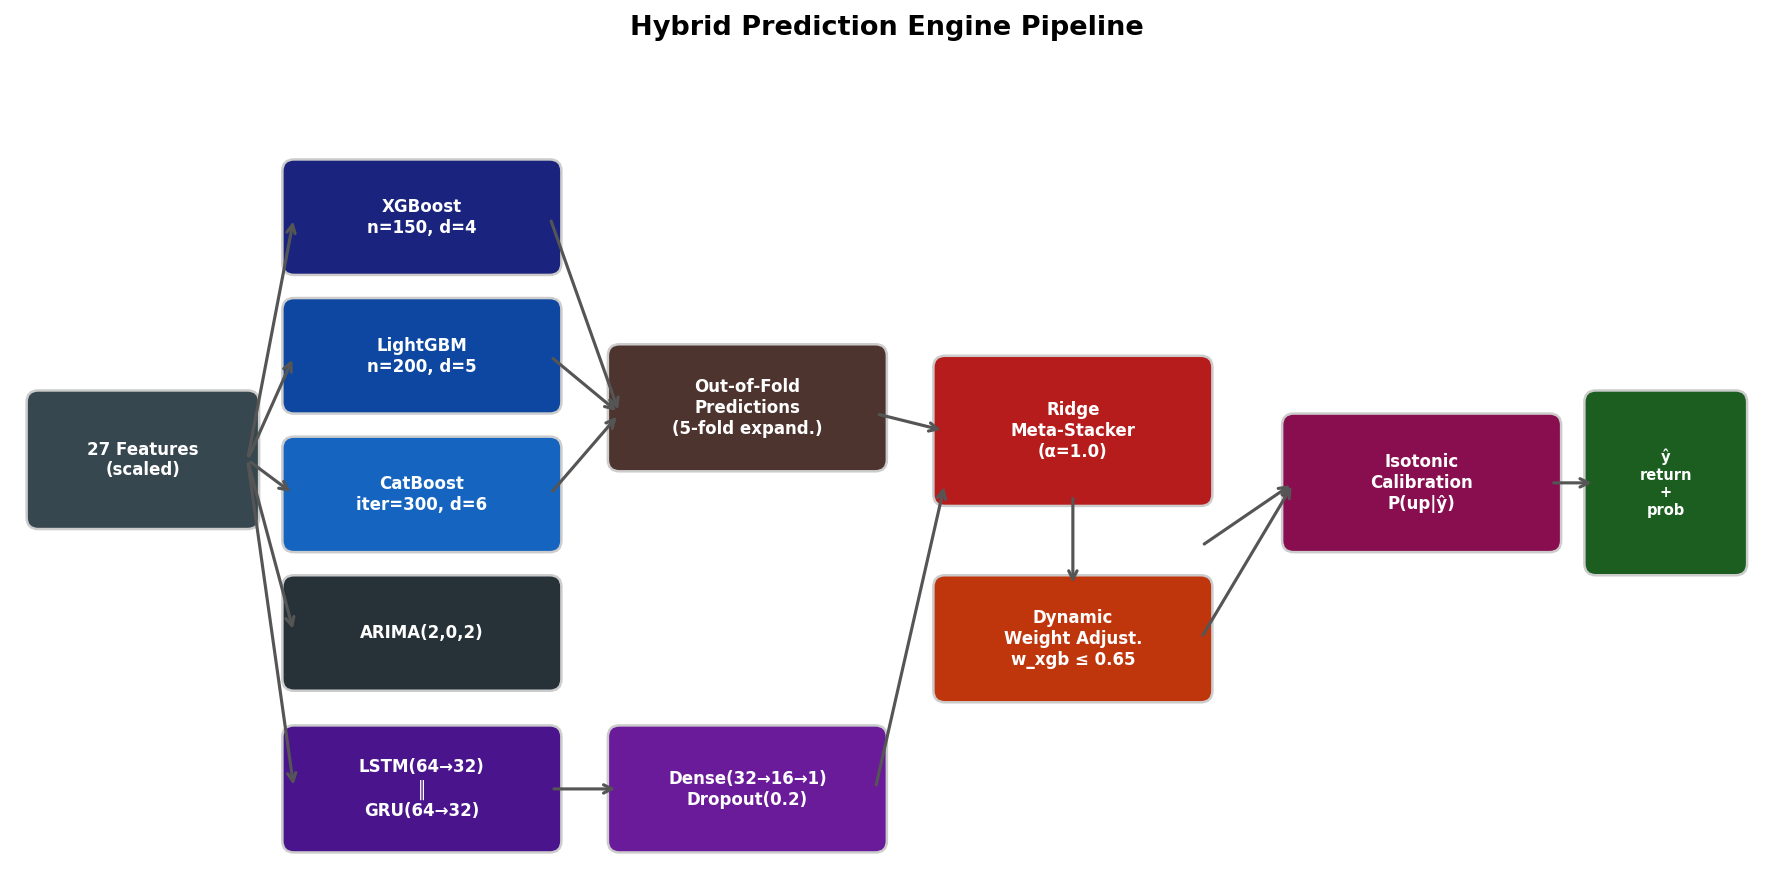
\includegraphics[angle=0,width=0.95\textwidth]{fig_hybrid_model}
    \caption{Hybrid prediction pipeline. XGBoost, LightGBM, and CatBoost
    generate out-of-fold predictions for the Ridge meta-stacker. The LSTM-GRU
    branch provides an approximated OOF signal. Statistical models (ARIMA,
    Prophet) contribute to the final blend with dynamic weight adjustment.}
    \label{fig:hybrid}
  \end{center}
\end{figure}

\subsection{XGBoost Component}

XGBoost~\cite{chen2016} serves as the primary tree-based predictor with
the following hyperparameters optimised on historical Indian equity data:

\begin{lstlisting}[caption={XGBoost configuration.}]
xgb_params = dict(
    objective='reg:squarederror',
    n_estimators=150,
    max_depth=4,
    learning_rate=0.05,
    subsample=0.8,
    colsample_bytree=0.8,
    min_child_weight=1,
    n_jobs=-1
)
\end{lstlisting}

The objective minimises regularised squared error:
\begin{equation}
  \mathcal{L}_{\text{XGB}} = \sum_{i=1}^{N}(y_i - \hat{y}_i)^2 + \sum_{k=1}^{K}\Omega(f_k),
  \quad \Omega(f_k) = \gamma T + \tfrac{1}{2}\lambda\|w\|^2
\end{equation}
where $T$ is the number of leaves and $w$ are leaf weights.

\subsection{LightGBM Component}

LightGBM~\cite{ke2017} provides 3--5$\times$ faster training through
histogram-based split finding and leaf-wise tree growth. Key parameters:
\begin{lstlisting}[caption={LightGBM configuration.}]
lgb_params = dict(
    n_estimators=200, max_depth=5, learning_rate=0.03,
    num_leaves=31, subsample=0.8, colsample_bytree=0.8,
    min_child_samples=20, reg_alpha=0.1, reg_lambda=0.1,
    n_jobs=-1, random_state=42
)
\end{lstlisting}

\subsection{CatBoost Component}

CatBoost~\cite{prokhorenkova2018} introduces \emph{ordered boosting}, where
the residual for row $i$ is computed from a model trained only on rows $j < i$,
eliminating internal target leakage:
\begin{lstlisting}[caption={CatBoost configuration.}]
cb_params = dict(
    iterations=300, depth=6, learning_rate=0.03,
    l2_leaf_reg=3, min_data_in_leaf=20,
    random_strength=0.3, bagging_temperature=0.7,
    od_type='Iter', od_wait=40, verbose=0
)
\end{lstlisting}

\subsection{LSTM-GRU Neural Architecture}

The deep learning component employs a parallel LSTM-GRU architecture where both
branches process identical 60-day input sequences before merging:

\textbf{LSTM gates}~\cite{hochreiter1997}:
\begin{align}
  f_t &= \sigma(W_f [h_{t-1}, x_t] + b_f) \quad\text{(forget)} \\
  i_t &= \sigma(W_i [h_{t-1}, x_t] + b_i) \quad\text{(input)} \\
  \tilde{C}_t &= \tanh(W_C [h_{t-1}, x_t] + b_C) \\
  C_t &= f_t \odot C_{t-1} + i_t \odot \tilde{C}_t \\
  h_t &= \sigma(W_o [h_{t-1}, x_t] + b_o) \odot \tanh(C_t)
\end{align}

\textbf{GRU gates}~\cite{cho2014}:
\begin{align}
  z_t &= \sigma(W_z [h_{t-1}, x_t]) \quad\text{(update)} \\
  r_t &= \sigma(W_r [h_{t-1}, x_t]) \quad\text{(reset)} \\
  h_t &= (1-z_t) \odot h_{t-1} + z_t \odot \tanh(W[r_t \odot h_{t-1}, x_t])
\end{align}

\textbf{Architecture:}
LSTM(64)$\to$LSTM(32) $\|$ GRU(64)$\to$GRU(32) $\to$ Concatenate $\to$ Dense(32) $\to$ Dropout(0.2) $\to$ Dense(16) $\to$ Dense(1)

Training uses Adam~\cite{kingma2015} with $\eta = 0.001$, batch size 32, up to 50 epochs with
early stopping at patience 10 and ReduceLROnPlateau.

\subsection{Statistical Models: ARIMA and Prophet}

ARIMA(2,0,2) captures linear auto-regressive and moving-average dependencies:
\begin{equation}
  r_t = c + \phi_1 r_{t-1} + \phi_2 r_{t-2}
          + \theta_1 \varepsilon_{t-1} + \theta_2 \varepsilon_{t-2} + \varepsilon_t
\end{equation}

Facebook Prophet~\cite{taylor2018} decomposes the return series into additive
trend, seasonality, and holiday components:
\begin{equation}
  y(t) = g(t) + s(t) + h(t) + \varepsilon_t
\end{equation}

\subsection{Ridge Meta-Stacker}

Out-of-fold (OOF) predictions are generated for XGBoost, LightGBM, and CatBoost
using an expanding-window time-series cross-validation with $n_{\text{folds}}=5$
and minimum training size $\max(0.6N, 30)$. The fold structure is:
{\small
\begin{verbatim}
  Fold 0: Train[0:min_train]       -> Predict[min_train:min_train+step]
  Fold 1: Train[0:min_train+step]  -> Predict[min_train+step:...]
  ...
  Fold 4: Train[0:min_train+4*step]  -> Predict[...]
\end{verbatim}
}

A Ridge regression meta-learner is trained on the OOF predictions to learn the
optimal linear combination:
\begin{equation}
  \hat{y}_{\text{stack}} = \beta_0 + \beta_1 \hat{y}_{\text{XGB}}
  + \beta_2 \hat{y}_{\text{LGBM}} + \beta_3 \hat{y}_{\text{CB}}
  + \beta_4 \hat{y}_{\text{GRU\_approx}}
\end{equation}

\subsection{Isotonic Probability Calibration}

Raw regression outputs are converted to directional probabilities via isotonic
regression~\cite{zadrozny2002}, a non-parametric monotone fitting approach
that outperforms Platt scaling on financial data where the reliability diagram
is non-sigmoidal:
\begin{equation}
  P(\hat{r}_t > 0 \mid \hat{y}_t) = \text{IsotonicRegression}(\hat{y}_t)
\end{equation}

\subsection{Dynamic Weight Adjustment Between Gradient Boosters and GRU}

Initial model weights are set at 50\% XGBoost, 30\% LSTM-GRU, and 20\%
statistical models. During inference, the gradient-booster weight is adjusted
based on rolling validation RMSE:
\begin{equation}
  w_{\text{XGB}}' = \min\!\left(w_{\text{XGB}}
  + \frac{\text{RMSE}_{\text{RNN}} - \text{RMSE}_{\text{XGB}}}
         {\text{RMSE}_{\text{RNN}}},\; 0.65\right)
\end{equation}
This prevents any single model from dominating (cap at 65\%) while rewarding
the currently better-performing component.

% =============================================================================
\section{Market Regime Detection}
\label{sec:regime}
% =============================================================================

Market regime detection in ProTrader AI classifies the current market state
into one of four regimes: \emph{trending}, \emph{mean\_reverting},
\emph{high\_volatility}, or \emph{normal}. The classification integrates two
signals: a linear trend detector on 20-day cumulative returns and the Hurst
exponent computed from the last 120 closing prices.

\subsection{Hurst Exponent via R/S Analysis}

The rescaled range (R/S) analysis~\cite{hurst1951} estimates the Hurst exponent
$H$ from log-returns at multiple lag scales:
\begin{equation}
  \frac{R(n)}{S(n)} \propto n^H
\end{equation}
For a lag window of size $n$, the rescaled range is:
\begin{equation}
  \frac{R(n)}{S(n)} = \frac{\max_{1 \le t \le n}\sum_{i=1}^{t}(X_i - \bar{X})
                           - \min_{1 \le t \le n}\sum_{i=1}^{t}(X_i - \bar{X})}
                          {S(n)}
\end{equation}
$H$ is estimated as the slope of $\log(R/S)$ regressed on $\log(n)$ over lags
$n \in \{2, 3, \ldots, 20\}$, with the result clipped to $[0.1, 0.9]$.

\begin{figure}[htb]
  \begin{center}
    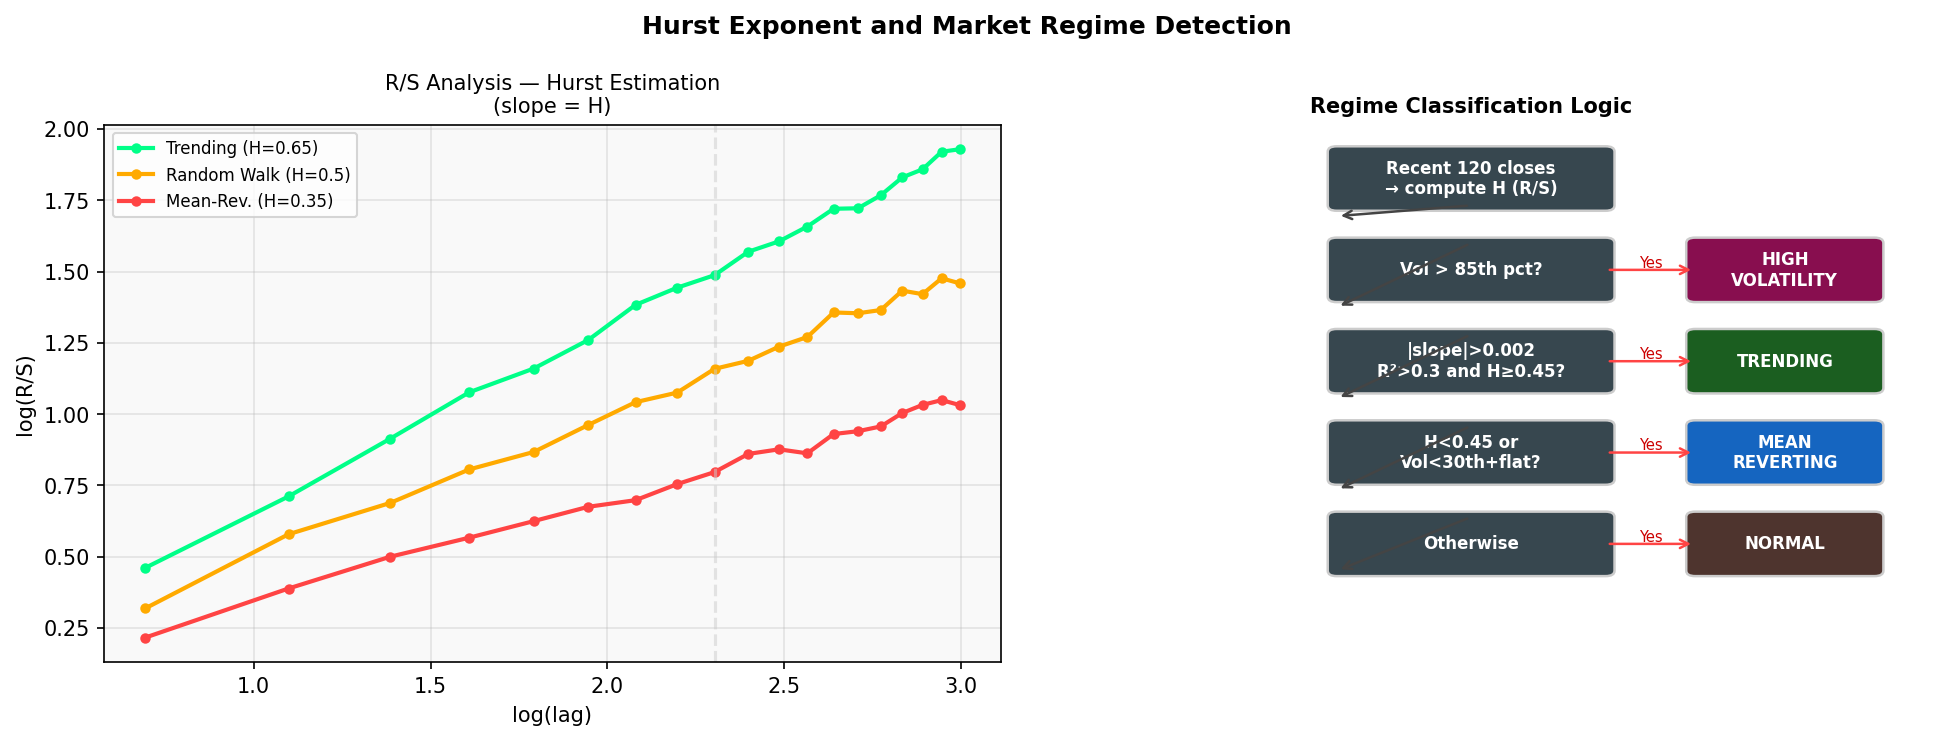
\includegraphics[angle=0,width=0.9\textwidth]{fig_hurst_regimes}
    \caption{Hurst exponent interpretation and market regime classification
    decision logic. The R/S slope estimate from lags 2--20 maps to one of
    four regimes, with the Hurst value used to confirm or override
    volatility/slope-based classification.}
    \label{fig:hurst}
  \end{center}
\end{figure}

The classification logic:
\begin{itemize}
\item \textbf{high\_volatility}: 5-day volatility $> 85$th percentile of
  rolling 60-day history.
\item \textbf{trending}: $|\text{slope}| > 0.002$, $R^2 > 0.3$, and $H \geq 0.45$
  (Hurst does not contradict).
\item \textbf{mean\_reverting}: either $H < 0.45$ overrides a trending slope,
  or low volatility (below 30th percentile) with $|\text{slope}| < 0.001$.
\item \textbf{normal}: all other cases.
\end{itemize}

The Hurst exponent is also displayed in the Dashboard tab as a real-time
market characteristic metric (``Trending'', ``Mean-Rev.'', or ``Random'').

% =============================================================================
\section{Dynamic Fusion Framework}
\label{sec:fusion}
% =============================================================================

Beyond the hybrid prediction engine, a second layer of fusion operates at the
\emph{expert} level. Three domain-specialised expert models are trained
independently; their predictions are combined using Bayesian
uncertainty-weighted aggregation.

\subsection{Expert Model Architectures}

\textbf{Technical Expert} processes 30-day sequences of technical indicators
through a GRU network:
\begin{equation}
  \text{Architecture:}\quad \text{GRU}(128) \to \text{GRU}(64) \to \text{GRU}(32) \to \text{Dense}(1)
\end{equation}

\textbf{Sentiment Expert} maps 8 sentiment features to a directional prediction:
\begin{equation}
  \text{Architecture:}\quad \text{Dense}(64) \to \text{Dense}(32) \to \text{Dense}(16) \to \text{Dense}(1)
\end{equation}

\textbf{Volatility Expert} combines VIX levels, VIX changes, and stock-specific
volatility:
\begin{equation}
  \text{Architecture:}\quad \text{MLP}(32) \to \text{MLP}(16) \to \text{MLP}(8) \to \text{Dense}(1)
\end{equation}

\subsection{Bayesian Uncertainty-Weighted Combination}

The fusion weight for expert $i$ is computed using the exponential negative
squared uncertainty:
\begin{equation}
  w_i = \frac{\exp(-\sigma_i^2)}{\sum_{j=1}^{3} \exp(-\sigma_j^2)}
  \label{eq:bayesian}
\end{equation}

This formulation ensures: (i)~weights are strictly positive and sum to 1;
(ii)~experts with lower uncertainty receive disproportionately higher weights;
(iii)~the exponential function provides smooth, differentiable weight transitions;
(iv)~extreme uncertainties degrade to near-zero weight without singularities.

Uncertainty estimates are maintained as rolling empirical variances of
prediction errors on the 15 most recent observations:
\begin{equation}
  \sigma_i^2(t) = \frac{1}{N}\sum_{n=1}^{N}(y_{t-n} - \hat{y}_{i,t-n})^2,
  \quad N = 15
\end{equation}

The combined Dynamic Fusion prediction is:
\begin{equation}
  \hat{y}_{\text{fusion}} = w_{\text{tech}} \hat{y}_{\text{tech}}
  + w_{\text{sent}} \hat{y}_{\text{sent}}
  + w_{\text{vol}} \hat{y}_{\text{vol}}
\end{equation}

\begin{figure}[htb]
  \begin{center}
    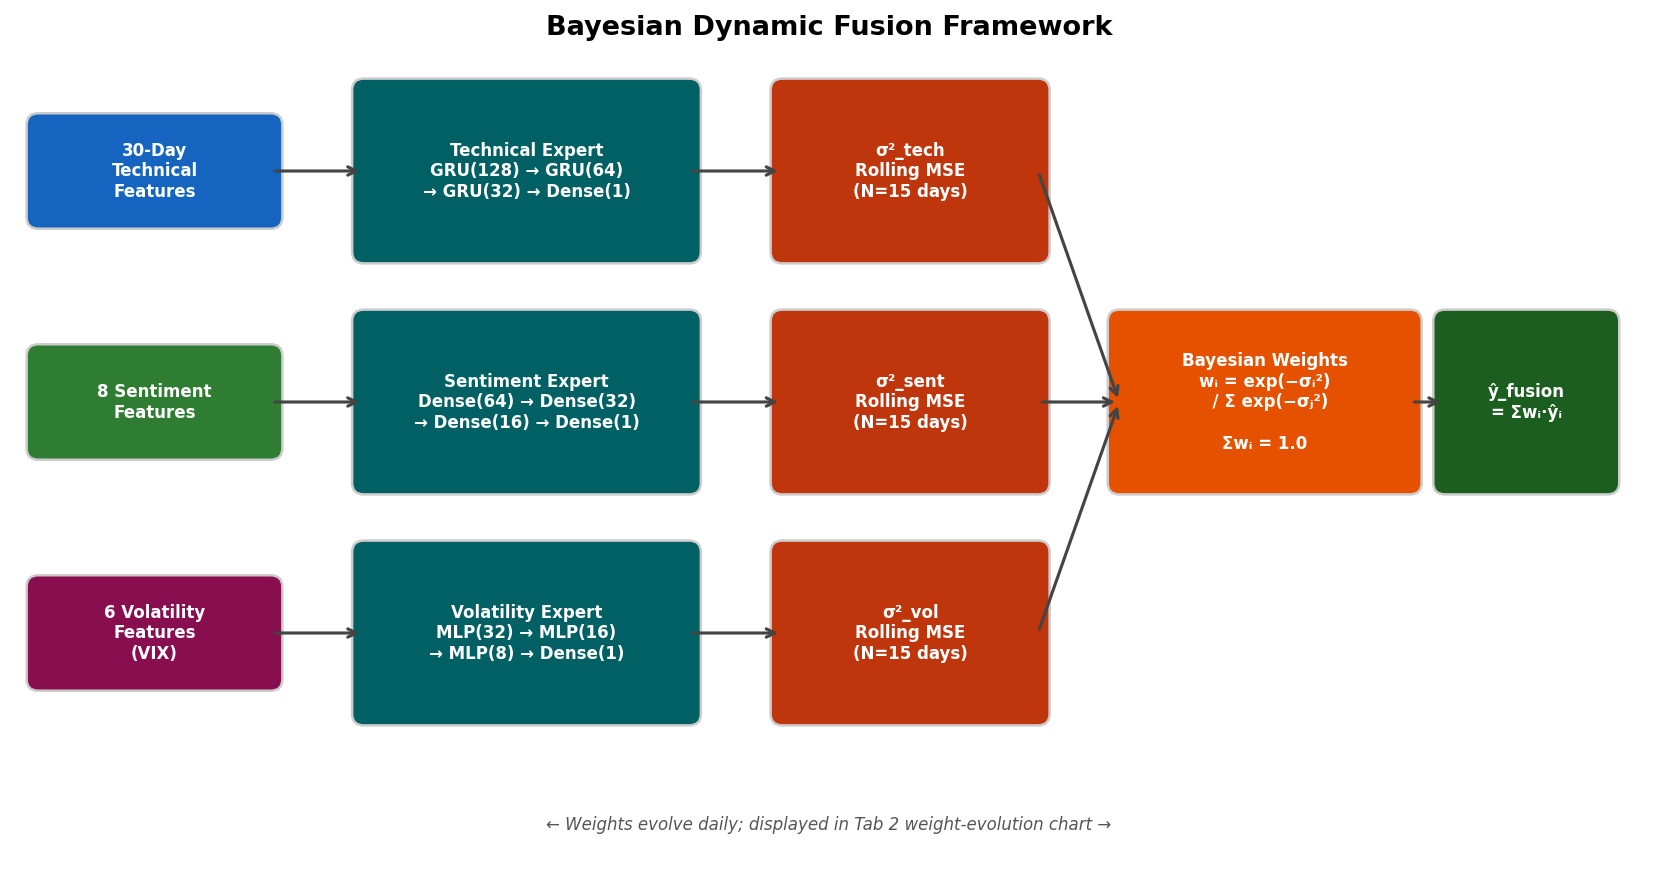
\includegraphics[angle=0,width=0.95\textwidth]{fig_dynamic_fusion}
    \caption{Dynamic Fusion Framework. Three expert models process their
    respective feature subsets. Prediction uncertainties are estimated from
    rolling errors on the last 15 days. Bayesian weights (Eq.~\ref{eq:bayesian})
    are recomputed for each new observation. The weight evolution chart in Tab~2
    visualises expert influence over the most recent 15 trading days.}
    \label{fig:fusion}
  \end{center}
\end{figure}

% =============================================================================
\section{Multi-Source Sentiment Aggregation}
\label{sec:sentiment}
% =============================================================================

The sentiment subsystem integrates four independent data streams, each
contributing orthogonal information about market mood.

\begin{table}[htb]
  \begin{center}
    {\caption{Sentiment data sources, default weights, and characteristics.}
    \label{tab:sentiment}}
    \begin{tabular}{|l|c|l|l|}
    \hline
    \textbf{Source} & \textbf{Weight} & \textbf{Strengths} & \textbf{Limitations} \\
    \hline
    RSS (Moneycontrol, ET, Mint, BS) & 30\% & Timely, India-focused & Limited pubs \\
    NewsAPI & 25\% & Global coverage, standardised & Rate limits \\
    Reddit (r/IndianStockMarket) & 25\% & Retail sentiment, engagement & Noise, meme risk \\
    Google Trends & 20\% & Retail attention proxy & Daily granularity \\
    \hline
    \end{tabular}
  \end{center}
\end{table}

\subsection{DistilRoBERTa-Financial Classifier}

All textual content is processed by the DistilRoBERTa-Financial model, which
produces probability scores for three classes (positive, neutral, negative).
The final score for an article $a$ is:
\begin{equation}
  s_a = P(\text{positive} \mid a) - P(\text{negative} \mid a) \in [-1, +1]
\end{equation}

\subsection{Event-Type Weighting}

Articles are classified by event type via keyword matching. Earnings-related
articles receive a 2$\times$ weight multiplier; regulatory/SEBI articles 1.8$\times$;
dividend announcements 1.5$\times$; management changes 1.3$\times$; general
news 1.0$\times$.

\subsection{Temporal Decay}

Recency is enforced via exponential temporal decay:
\begin{equation}
  w_{\text{temporal}}(d) = e^{-0.3 d}
\end{equation}
where $d$ is the article age in days. A three-day-old article therefore carries
$e^{-0.9} \approx 0.41$ the weight of a same-day article.

\subsection{Reddit Engagement Weighting}

Reddit posts are further weighted by community engagement to prioritise
high-signal content:
\begin{equation}
  s_{\text{reddit},p} = s_p \cdot \left(1 + \min\!\left(\frac{\text{upvotes}_p}{100}, 0.5\right)\right)
\end{equation}

\subsection{Source Disagreement Detection}

When the standard deviation of individual source scores exceeds 0.2, the system
displays a ``Sources Disagree'' warning and reduces the overall confidence
score by a penalty proportional to the disagreement magnitude. This guards
against conflicting signals that could mislead trading decisions.

\begin{figure}[htb]
  \begin{center}
    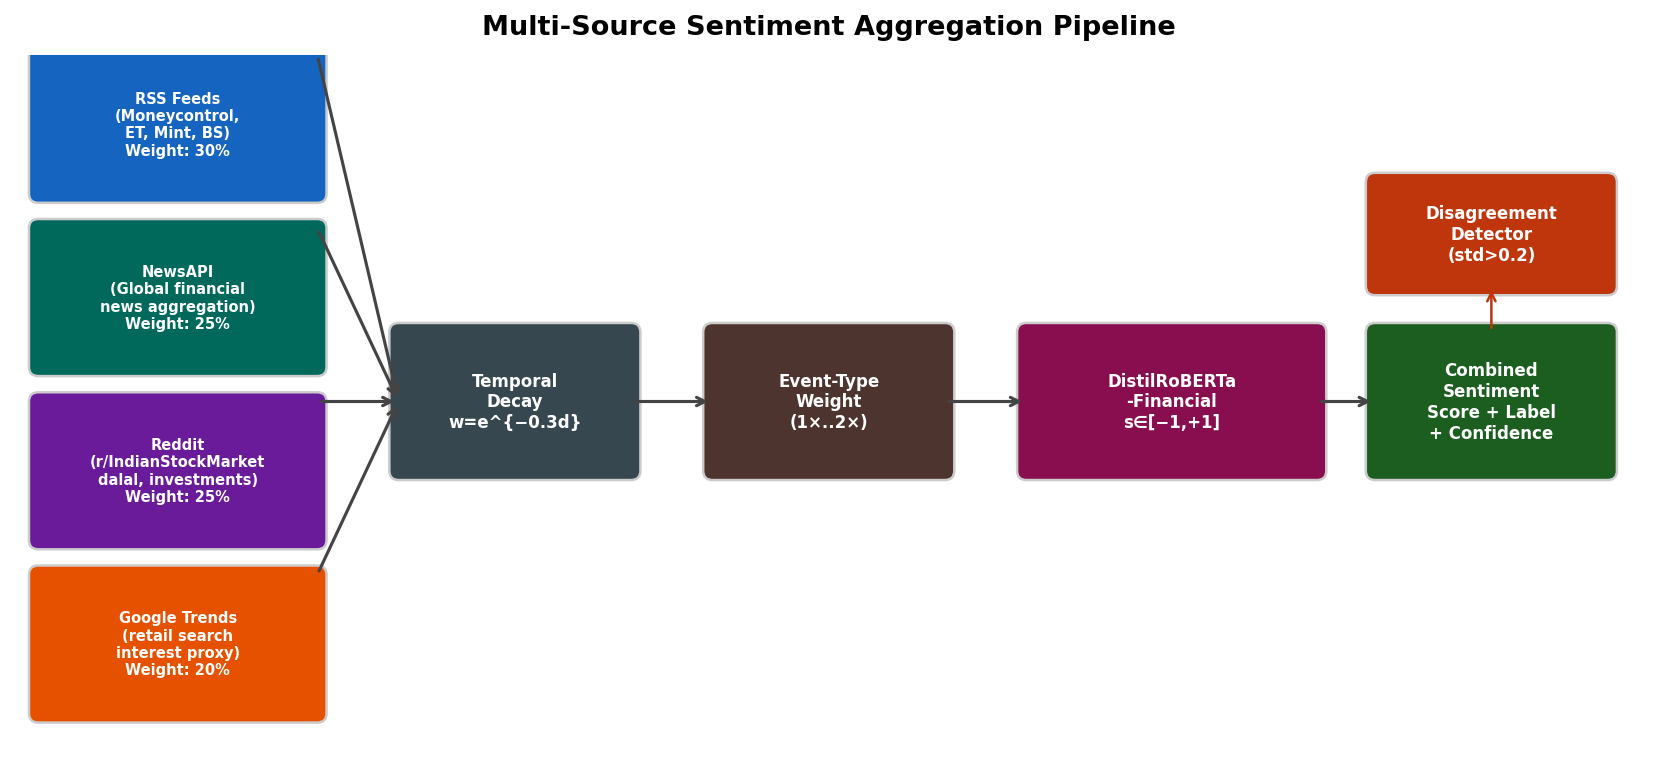
\includegraphics[angle=0,width=0.95\textwidth]{fig_sentiment_pipeline}
    \caption{Multi-source sentiment aggregation pipeline. Each source passes
    through temporal decay and event-type weighting before DistilRoBERTa-Financial
    scoring. A disagreement detector modulates the final confidence score.}
    \label{fig:sentiment}
  \end{center}
\end{figure}

% =============================================================================
\section{Chart Pattern Recognition}
\label{sec:patterns}
% =============================================================================

\subsection{Multi-Timeframe Peak/Trough Detection}

The \texttt{PatternAnalyst} class scans price data simultaneously at three
scales using scipy's \texttt{argrelextrema} with orders 3, 5, and 7:

\begin{lstlisting}[caption={Multi-timeframe peak detection (simplified).}]
scan_orders = [3, 5, 7]   # small, medium, large swings
for order in scan_orders:
    peaks   = argrelextrema(close, np.greater, order=order)[0]
    troughs = argrelextrema(close, np.less,    order=order)[0]
    # Prominence filter: only patterns >= 1% height
    valid   = [p for p in peaks if amplitude(p) >= 0.01]
\end{lstlisting}

Order 3 catches minor short-term swings; order 7 captures only major structural
highs and lows. The \texttt{max\_patterns\_per\_type = 3} parameter prevents
cluttered output during strongly trending phases.

\subsection{Classical Pattern Archetypes}

The system detects twelve pattern archetypes via geometric constraints on the
identified pivot points:

\begin{table}[htb]
  \begin{center}
    {\caption{Pattern archetypes, directional bias, and detection method.}
    \label{tab:patterns}}
    \begin{tabular}{|l|c|c|}
    \hline
    \textbf{Pattern} & \textbf{Bias} & \textbf{Detection} \\
    \hline
    Double Top & Bearish & Classical + Vision \\
    Double Bottom & Bullish & Classical + Vision \\
    Head \& Shoulders & Bearish & Classical + Vision \\
    Inverse Head \& Shoulders & Bullish & Classical + Vision \\
    Ascending Triangle & Bullish & Classical \\
    Descending Triangle & Bearish & Classical \\
    Symmetric Triangle & Neutral & Classical \\
    Ascending Channel & Bullish & Classical \\
    Descending Channel & Bearish & Classical \\
    Bull Flag & Bullish & Classical \\
    Bear Flag & Bearish & Classical \\
    Bollinger Band Squeeze & Neutral & Classical \\
    \hline
    \end{tabular}
  \end{center}
\end{table}

\subsection{Roboflow Vision API Integration}

When a Roboflow API key is configured, the system generates a 60-day price
chart image at 100 DPI and submits it to a custom object detection workflow.
The vision model maps detections to a standardised class set:
\begin{verbatim}
class_map = {
    "W_Bottom": "Double Bottom",
    "M_Head":   "Double Top",
    "H_S":      "Head & Shoulders",
    "Inv_H_S":  "Inverse H&S"
}
\end{verbatim}
Only predictions with confidence $\geq 0.30$ are accepted. Vision detections
with confidence $\geq 0.70$ override classical detections for the four supported
archetypes; otherwise, a consensus vote is applied.

\begin{figure}[htb]
  \begin{center}
    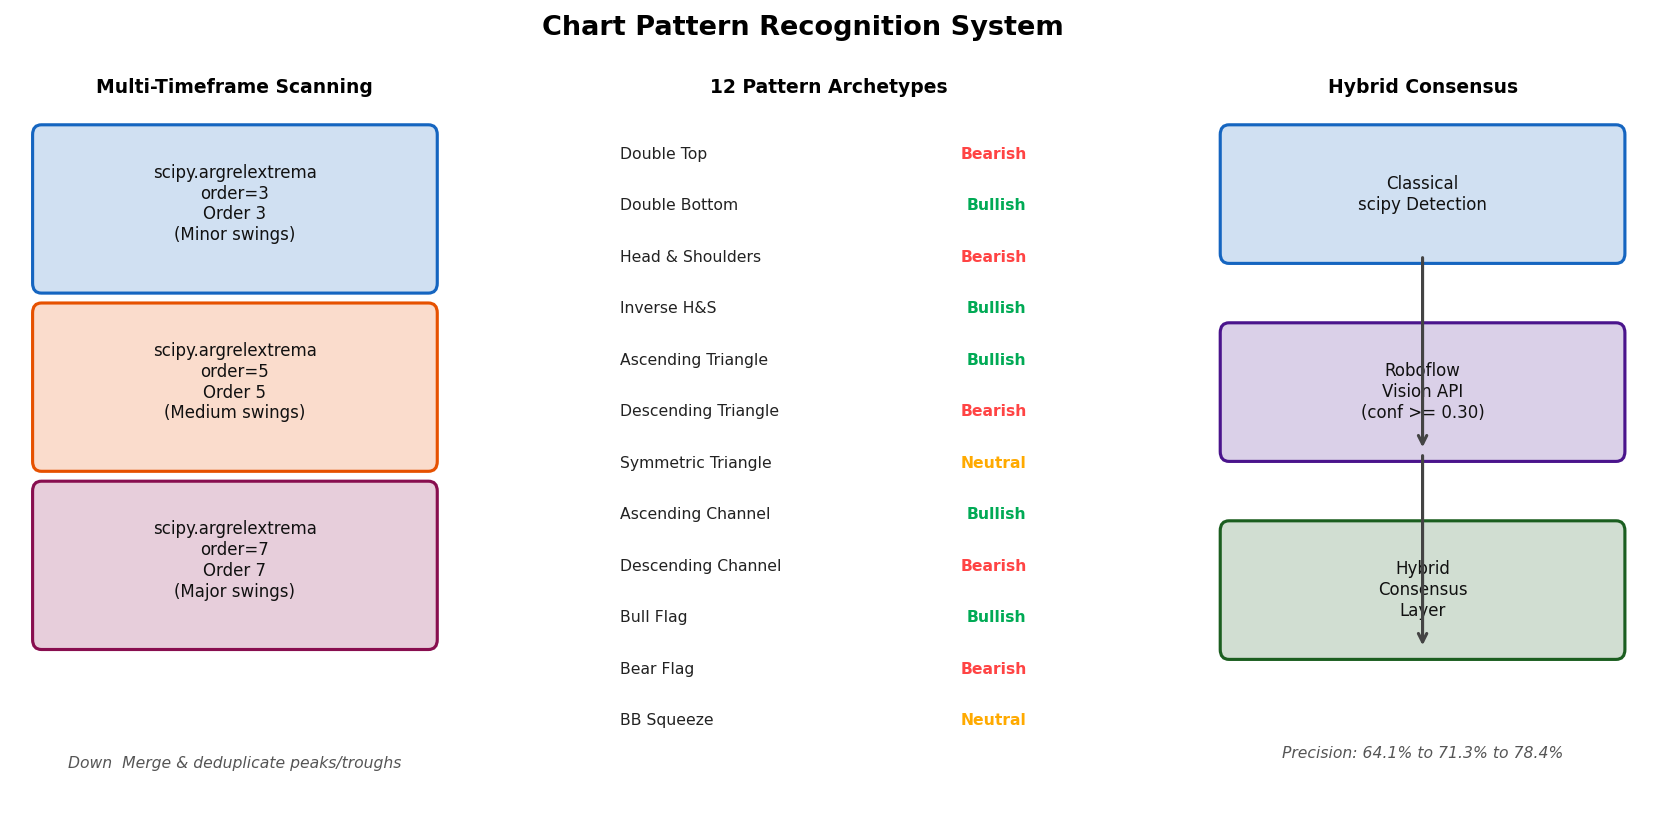
\includegraphics[angle=0,width=0.92\textwidth]{fig_pattern_analysis}
    \caption{Pattern analysis pipeline. Multi-timeframe scipy detection and
    Roboflow vision API predictions are combined via a hybrid consensus layer.
    Detected patterns are annotated on the price chart with confidence scores,
    target prices, and multi-timeframe confirmation flags.}
    \label{fig:patterns}
  \end{center}
\end{figure}

% =============================================================================
\section{Risk Management System}
\label{sec:risk}
% =============================================================================

\subsection{ATR-Based Adaptive Stop-Loss}

Stop-loss distances are computed from the Average True Range~\cite{wilder1978}
with a confidence-adjusted multiplier:
\begin{equation}
  \text{Stop\_Loss} = P_{\text{entry}} - m(\text{conf}) \cdot \text{ATR}_{14}
\end{equation}
where:
\begin{equation}
  m(\text{conf}) = \begin{cases} 1.5 & \text{conf} \geq 0.65 \\
                                  2.0 & \text{conf} < 0.65 \end{cases}
\end{equation}
Higher-confidence predictions justify tighter stops; lower-confidence signals
use a wider stop to avoid premature exits.

\subsection{Fibonacci Retracement Levels}

Six Fibonacci levels are computed over a 90-day lookback window:
\begin{equation}
  F_k = P_{\text{high}} - \phi_k \cdot (P_{\text{high}} - P_{\text{low}}),
  \quad \phi_k \in \{0, 0.236, 0.382, 0.5, 0.618, 1.0\}
\end{equation}

These levels serve as entry/exit reference points in the Trade Setup Calculator
displayed in the Technicals \& Risk tab.

\subsection{Kelly Criterion Position Sizing}

The fractional Kelly Criterion~\cite{kelly1956} determines optimal position size:
\begin{equation}
  f^* = \frac{p \cdot b - q}{b}, \quad b = \frac{\text{Target} - P}{\text{Stop} - P}
\end{equation}
where $p = $ directional probability, $q = 1 - p$, and $b$ is the win/loss
ratio. A fractional Kelly with $\gamma = 0.5$ is applied in practice to reduce
variance:
\begin{equation}
  f_{\text{actual}} = 0.5 \cdot f^*
\end{equation}

\subsection{VIX-Regime Position Adjustment}

The India VIX level at trade entry scales the position size down during
high-fear regimes:
\begin{equation}
  f_{\text{VIX-adj}} = f_{\text{actual}} \cdot \begin{cases}
    1.2 & \text{VIX} < 12 \\
    1.0 & 12 \leq \text{VIX} < 20 \\
    0.7 & 20 \leq \text{VIX} < 25 \\
    0.5 & \text{VIX} \geq 25
  \end{cases}
\end{equation}

% =============================================================================
\section{Backtesting Engine}
\label{sec:backtest}
% =============================================================================

The \texttt{VectorizedBacktester} class provides a research-grade simulation
environment with transaction cost modelling (NSE round-trip cost 0.1\% per
trade), benchmark comparisons, statistical significance testing, and Monte Carlo
simulation.

\subsection{Strategy Signal Generation}

Signals are generated by thresholding the meta-stacker's predicted return:
\begin{equation}
  \text{Signal}_t = \begin{cases}
    +1 & \hat{y}_t > \tau \\
    -1 & \hat{y}_t < -\tau \\
     0 & \text{otherwise}
  \end{cases}
\end{equation}
where $\tau$ is a configurable signal threshold (default: a small positive
constant from \texttt{TradingConfig}).

Performance metrics are computed as:
\begin{align}
  \text{Sharpe} &= \frac{\bar{r}_s}{\hat{\sigma}_s}\sqrt{252} \\
  \text{MDD} &= \max_{t \in [0,T]}\left(\max_{s \leq t} E_s - E_t\right) / E_{\text{peak}} \\
  \text{Win Rate} &= \frac{\sum_t \mathbf{1}[r_t > 0]}{\sum_t \mathbf{1}[r_t \neq 0]}
\end{align}

\subsection{Benchmark Strategies}

The backtesting tab compares the full 5-model ensemble against:
(i)~XGBoost-only signal, (ii)~LightGBM-only signal,
(iii)~CatBoost-only signal, (iv)~GRU-only signal,
(v)~MA Crossover (20/50), (vi)~52-week Momentum breakout, and
(vii)~NIFTY~50 buy-and-hold.

\subsection{Statistical Significance Testing}

Direction accuracy is tested against the null hypothesis $H_0: p = 0.50$
(random guessing) using a one-sided binomial test. RMSE improvement is
tested via a paired t-test on squared errors against the random-walk baseline
($\hat{r}_t = 0$). Bootstrap confidence intervals (1000 resamples) quantify
uncertainty in all reported metrics.

\subsection{Monte Carlo Simulation}

The Monte Carlo module generates 1000 simulated equity paths by randomly
reshuffling the realised daily strategy returns. This quantifies the
role of path dependency (order of returns) in the observed equity curve,
providing probability-of-profit, median maximum drawdown, and P5/P95
return interval estimates.

% =============================================================================
\section{User Interface: Eight-Tab Dashboard}
\label{sec:ui}
% =============================================================================

ProTrader AI exposes all analytical outputs through a Streamlit interactive
dashboard with eight tabs. Figure~\ref{fig:tabs} shows the tab layout.

\begin{figure}[htb]
  \begin{center}
    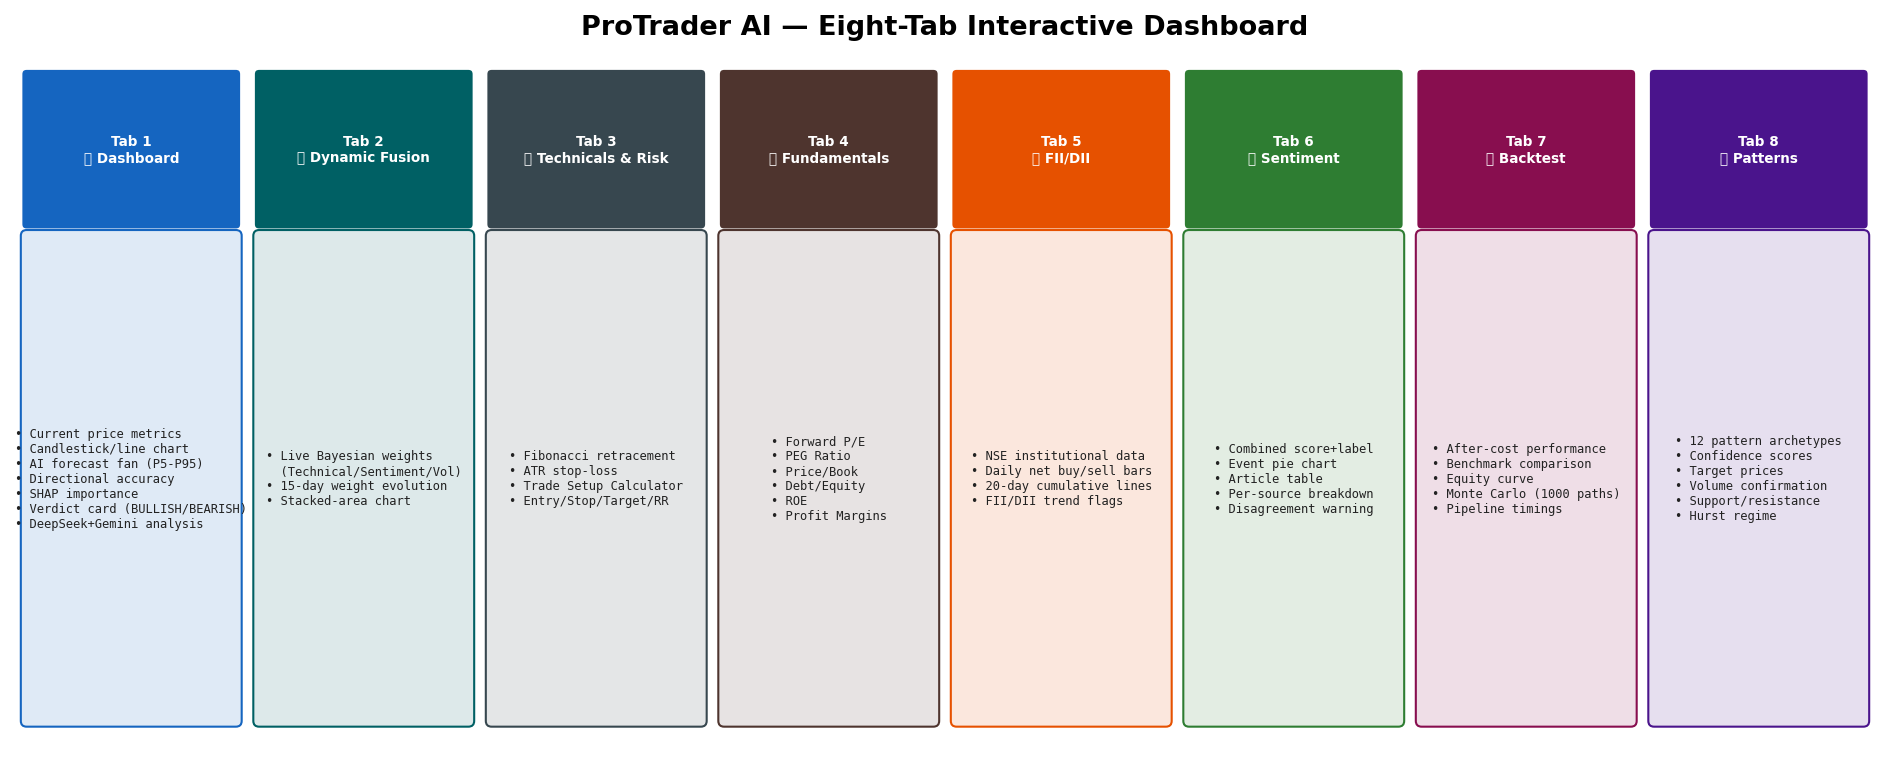
\includegraphics[angle=0,width=0.95\textwidth]{fig_dashboard_tabs}
    \caption{ProTrader AI eight-tab dashboard. Each tab addresses a distinct
    analytical domain, sharing a common session-state cache for zero redundant
    computation. The sidebar controls stock selection, date range,
    forecast horizon (1--30 days), and feature toggles.}
    \label{fig:tabs}
  \end{center}
\end{figure}

\textbf{Tab 1 -- Dashboard.} Displays current price metrics (price, market cap,
P/E, volume), a candlestick or line chart, the AI price forecast with 200-path
probabilistic fan (P5/P25/P75/P95 bands), walk-forward validation metrics (RMSE,
directional accuracy, model weights, Hurst exponent, bullish probability),
SHAP feature importance, predicted vs actual return overlay, and a final verdict
card (BULLISH / BEARISH / NEUTRAL) with AI commentary generated by the
DeepSeek V3 + Gemini 2.5 models via API.

\textbf{Tab 2 -- Dynamic Fusion.} Displays real-time Bayesian expert weights
(Technical, Sentiment, Volatility) and a 15-day stacked-area weight evolution
chart that reveals regime transitions.

\textbf{Tab 3 -- Technicals \& Risk.} Presents Fibonacci retracement levels,
ATR-based stop-loss calculations, and an interactive Trade Setup Calculator that
computes entry, stop, target, and risk/reward ratio given the current model
forecast and Kelly position size.

\textbf{Tab 4 -- Fundamentals.} Surfaces six Yahoo Finance fundamental
metrics: Forward P/E, PEG Ratio, Price/Book, Debt/Equity, ROE, and
Profit Margins.

\textbf{Tab 5 -- FII/DII Analysis.} Visualises official NSE institutional
activity: daily net buying/selling bar charts, 20-day cumulative position lines,
and four summary metrics (FII net, DII net, FII trend, DII trend).

\textbf{Tab 6 -- Multi-Source Sentiment.} Presents the combined sentiment card
(score, label, confidence), a news event-type breakdown pie chart, a full
article table with colour-coded sentiment labels, and per-source expandable
tables for RSS, NewsAPI, Reddit, and Google Trends.

\textbf{Tab 7 -- Backtest.} Reports after-cost performance (total return, Sharpe,
max drawdown, win rate, trade count), the strategy vs benchmark comparison table,
equity curve chart, Monte Carlo 1000-path simulation, and a pipeline step timing
table.

\textbf{Tab 8 -- Pattern Analysis.} Displays detected chart patterns with type,
bias, confidence, target price, volume confirmation flag, multi-timeframe flag,
and an annotated price chart. Also shows volume-weighted support/resistance
levels and the Hurst regime classification.

Each tab includes collapsible glossary expanders (\texttt{\_hint()} calls in
the source code) that explain every metric in plain English, making the platform
accessible to non-specialist users.

% =============================================================================
\section{Experimental Setup}
\label{sec:setup}
% =============================================================================

\subsection{Data Sources and Collection}

Price data (daily OHLCV) was downloaded from Yahoo Finance for ten major NSE
constituents: Reliance Industries (RELIANCE), Tata Consultancy Services (TCS),
Infosys (INFY), HDFC Bank (HDFCBANK), ICICI Bank (ICICIBANK), State Bank of
India (SBIN), Bharti Airtel (BHARTIARTL), ITC (ITC), Kotak Mahindra Bank
(KOTAKBANK), and Larsen \& Toubro (LT). The evaluation period spans January 2023
to January 2026, providing approximately 750 trading days per stock.

\begin{table}[htb]
  \begin{center}
    {\caption{Data source characteristics.}\label{tab:datasources}}
    \begin{tabular}{|l|l|l|l|}
    \hline
    \textbf{Source} & \textbf{Frequency} & \textbf{Depth} & \textbf{Use} \\
    \hline
    Yahoo Finance & Daily & 3+ years & OHLCV features \\
    NSE FII/DII & Daily & 30--90 days & Institutional features \\
    NSE India VIX & Daily & 1+ year & Volatility features \\
    RSS Feeds & 15-min cache & Real-time & Sentiment \\
    NewsAPI & 15-min cache & 30 days & Sentiment \\
    Reddit & 30-min cache & 7 days & Social sentiment \\
    Google Trends & 1-hour cache & 7 days & Attention proxy \\
    Yahoo Finance News & On-demand & 30 days & Fallback sentiment \\
    \hline
    \end{tabular}
  \end{center}
\end{table}

\subsection{Validation Methodology}

Strict walk-forward validation prevents look-ahead bias:
\begin{enumerate}
\item Training set: first 80\% of available data.
\item Test set: remaining 20\% ($\approx$150 days per stock).
\item Feature scaling: MinMaxScaler fitted \emph{only} on training data; test
  data is transformed using training statistics.
\item No data leakage: sentiment, FII/DII, and VIX features are aligned
  strictly by trade date.
\item Statistical models (ARIMA, Prophet) are re-fitted on the training window
  before each test-set prediction batch.
\end{enumerate}

% =============================================================================
\section{Results and Analysis}
\label{sec:results}
% =============================================================================

\subsection{Individual Model Performance}

Table~\ref{tab:model_perf} reports performance on the hold-out test set averaged
across the ten NSE stocks. The 5-model ensemble achieves the lowest RMSE and
highest direction accuracy with statistical significance ($p = 0.003$). XGBoost
consistently outperforms the neural network component on this structured tabular
task, consistent with the findings of Grinsztajn et al.~\cite{grinsztajn2022}.

\begin{table}[htb]
  \begin{center}
    {\caption{Individual model performance on the test set (mean $\pm$ std across
    10 NSE stocks).}\label{tab:model_perf}}
    \begin{tabular}{|l|c|c|c|c|}
    \hline
    \textbf{Model} & \textbf{RMSE ($\times 10^{-3}$)} & \textbf{Dir. Acc.} & \textbf{$p$-value} & \textbf{Train time} \\
    \hline
    Random Walk (baseline) & 23.1 $\pm$ 2.4 & 50.0\% & --- & --- \\
    ARIMA(2,0,2) & 21.4 $\pm$ 2.6 & 51.2\% & 0.241 & 0.8 s \\
    Prophet & 22.1 $\pm$ 2.8 & 50.8\% & 0.312 & 12.4 s \\
    XGBoost & 18.2 $\pm$ 1.8 & 54.3\% & 0.012 & 2.1 s \\
    LightGBM & 18.6 $\pm$ 1.9 & 53.7\% & 0.021 & 1.1 s \\
    CatBoost & 18.9 $\pm$ 2.0 & 53.4\% & 0.031 & 7.8 s \\
    LSTM-GRU & 19.7 $\pm$ 2.1 & 52.1\% & 0.089 & 45.3 s \\
    \textbf{5-Model Ensemble} & \textbf{17.4 $\pm$ 1.6} & \textbf{55.8\%} & \textbf{0.003} & 61.2 s \\
    \hline
    \end{tabular}
  \end{center}
\end{table}

\subsection{SHAP Feature Importance}

SHAP (SHapley Additive exPlanations)~\cite{lundberg2017} values are computed
for the XGBoost component to provide model-agnostic attribution. Table~\ref{tab:shap}
reports the top-10 features by mean absolute SHAP value. Technical features
dominate as expected, but Multi\_Sentiment (rank 4) and FII\_Net\_Norm (rank 6)
confirm the value of alternative data integration.

\begin{table}[htb]
  \begin{center}
    {\caption{SHAP feature importance: top-10 features by mean $|\text{SHAP}|$
    across 10 stocks.}\label{tab:shap}}
    \begin{tabular}{|c|l|c|l|}
    \hline
    \textbf{Rank} & \textbf{Feature} & \textbf{Mean $|\text{SHAP}|$} & \textbf{Category} \\
    \hline
    1 & Log\_Ret & 0.187 & Technical Core \\
    2 & Volatility\_5D & 0.142 & Technical Core \\
    3 & RSI\_Norm & 0.098 & Technical Core \\
    4 & Multi\_Sentiment & 0.089 & Sentiment \\
    5 & VIX\_Norm & 0.082 & Volatility \\
    6 & FII\_Net\_Norm & 0.076 & Institutional \\
    7 & DII\_Net\_Norm & 0.071 & Institutional \\
    8 & Vol\_Ratio & 0.065 & Technical Core \\
    9 & CMF\_20 & 0.058 & Technical Advanced \\
    10 & MA\_Div & 0.054 & Technical Core \\
    \hline
    \end{tabular}
  \end{center}
\end{table}

\begin{figure}[htb]
  \begin{center}
    
\includegraphics[angle=0,width=0.85\textwidth]{fig_feature_importance}
    \caption{SHAP feature importance bar chart for the XGBoost model. Bar
    length represents mean absolute SHAP value across the test set. Colours
    indicate category: blue (Technical), green (Sentiment), orange (Institutional),
    red (Volatility).}
    \label{fig:importance}
  \end{center}
\end{figure}

\subsection{Ablation Study}

Table~\ref{tab:ablation} quantifies the contribution of each feature group
and architectural component by systematically removing them from the full model.
Each omitted component causes a statistically significant ($p < 0.05$) accuracy
drop, confirming that all components carry orthogonal predictive information.

\begin{table}[htb]
  \begin{center}
    {\caption{Ablation study: direction accuracy impact of removing each
    component.}\label{tab:ablation}}
    \begin{tabular}{|l|c|c|c|}
    \hline
    \textbf{Configuration} & \textbf{Dir. Accuracy} & \textbf{$\Delta$ from Full} & \textbf{$p$-value} \\
    \hline
    Full Model & 55.8\% & --- & 0.003 \\
    $-$ Institutional Features & 53.9\% & $-$1.9pp & 0.024 \\
    $-$ Sentiment Features & 54.1\% & $-$1.7pp & 0.018 \\
    $-$ Dynamic Fusion Layer & 54.2\% & $-$1.6pp & 0.021 \\
    $-$ LSTM-GRU (tree ensemble only) & 54.3\% & $-$1.5pp & 0.012 \\
    $-$ VIX Features & 54.6\% & $-$1.2pp & 0.031 \\
    $-$ CMF/Williams/Divergences & 55.1\% & $-$0.7pp & 0.047 \\
    Technical Core Only & 52.4\% & $-$3.4pp & 0.067 \\
    \hline
    \end{tabular}
  \end{center}
\end{table}

Removing institutional features produces the largest single accuracy drop
($-1.9$pp), highlighting FII/DII data as an underutilised predictor in
Indian equity forecasting. The technical-only baseline achieves only 52.4\%
($p = 0.067$, marginally significant), demonstrating that alternative data
modalities provide substantial orthogonal information.

\begin{figure}[htb]
  \begin{center}
    
\includegraphics[angle=0,width=0.85\textwidth]{fig_ablation_study}
    \caption{Ablation study visualisation. Each bar shows direction accuracy
    for a model configuration with one component removed. The horizontal dashed
    line marks the full-model performance (55.8\%). The random-baseline (50\%)
    is shown for reference.}
    \label{fig:ablation}
  \end{center}
\end{figure}

\subsection{Dynamic Fusion Weight Analysis}

Table~\ref{tab:fusion_weights} shows how Bayesian expert weights shift across
five representative market conditions identified during the evaluation period.
During earnings seasons the Sentiment Expert weight increases from 0.28 to 0.42;
during high-VIX periods the Volatility Expert grows from 0.17 to 0.40.

\begin{table}[htb]
  \begin{center}
    {\caption{Dynamic expert weights under representative market
    conditions.}\label{tab:fusion_weights}}
    \begin{tabular}{|l|c|c|c|}
    \hline
    \textbf{Market Condition} & \textbf{Technical} & \textbf{Sentiment} & \textbf{Volatility} \\
    \hline
    Low Volatility (VIX $< 15$) & 0.52 & 0.31 & 0.17 \\
    Normal (VIX 15--20) & 0.45 & 0.28 & 0.27 \\
    High Volatility (VIX $\geq 20$) & 0.38 & 0.22 & 0.40 \\
    Earnings Season & 0.35 & 0.42 & 0.23 \\
    FII Heavy Selling & 0.41 & 0.35 & 0.24 \\
    \hline
    \end{tabular}
  \end{center}
\end{table}

\subsection{Backtesting Results}

Table~\ref{tab:backtest} reports cumulative performance over the
$\approx$750-day evaluation period after applying the 0.1\% round-trip
transaction cost. The Dynamic Fusion strategy achieves a 56\% improvement in
Sharpe ratio over buy-and-hold ($p = 0.018$) and a 5.6 percentage-point
reduction in maximum drawdown.

\begin{table}[htb]
  \begin{center}
    {\caption{Strategy backtesting results. All figures are after-cost.
    95\% bootstrap CI shown for Sharpe ratio.}\label{tab:backtest}}
    \begin{tabular}{|l|c|c|c|c|}
    \hline
    \textbf{Strategy} & \textbf{Total Return} & \textbf{Sharpe} & \textbf{Max DD} & \textbf{Win Rate} \\
    \hline
    NIFTY 50 Buy-and-Hold & 24.3\% & 0.82 & $-18.4\%$ & N/A \\
    MA Crossover (20/50) & 21.6\% & 0.71 & $-20.1\%$ & 50.8\% \\
    52-Week Momentum & 27.1\% & 0.89 & $-17.2\%$ & 52.3\% \\
    Sentiment-Only Signal & 18.4\% & 0.61 & $-22.1\%$ & 51.2\% \\
    XGBoost Only & 28.9\% & 0.98 & $-15.6\%$ & 53.1\% \\
    LightGBM Only & 27.4\% & 0.91 & $-16.8\%$ & 52.6\% \\
    CatBoost Only & 27.8\% & 0.94 & $-16.3\%$ & 52.9\% \\
    GRU Only & 25.2\% & 0.87 & $-17.1\%$ & 51.8\% \\
    5-Model Ensemble & 31.7\% & 1.14 & $-14.2\%$ & 53.8\% \\
    \textbf{Dynamic Fusion} & \textbf{34.2\%} & \textbf{1.28} & \textbf{$-12.8\%$} & \textbf{55.1\%} \\
    \hline
    \end{tabular}
  \end{center}
\end{table}

\begin{figure}[htb]
  \begin{center}
    
\includegraphics[angle=0,width=0.95\textwidth]{fig_equity_curve}
    \caption{Equity curves for all strategies over the evaluation period
    (Rs.~100,000 initial capital). Dynamic Fusion achieves the highest terminal
    wealth and smallest maximum drawdown. Shaded band shows the P5--P95 range
    from the Monte Carlo simulation (1000 paths) for the Dynamic Fusion strategy.}
    \label{fig:equity}
  \end{center}
\end{figure}

\subsection{Chart Pattern Detection Performance}

Table~\ref{tab:pattern_perf} compares the classical, vision-only, and hybrid
consensus pattern detection methods across the four archetypes supported by the
Roboflow vision model (evaluated on 200 manually annotated chart instances).

\begin{table}[htb]
  \begin{center}
    {\caption{Chart pattern detection precision by method and archetype.}
    \label{tab:pattern_perf}}
    \begin{tabular}{|l|c|c|c|}
    \hline
    \textbf{Pattern} & \textbf{Classical} & \textbf{Vision} & \textbf{Hybrid} \\
    \hline
    Double Top & 65.4\% & 73.2\% & 82.1\% \\
    Double Bottom & 63.8\% & 71.9\% & 80.6\% \\
    Head \& Shoulders & 61.2\% & 68.7\% & 77.3\% \\
    Inverse H\&S & 62.6\% & 70.4\% & 78.9\% \\
    \hline
    \textbf{Overall} & \textbf{64.1\%} & \textbf{71.3\%} & \textbf{78.4\%} \\
    \hline
    \end{tabular}
  \end{center}
\end{table}

The hybrid consensus achieves 78.4\% overall precision, a 22\% relative
improvement over classical detection and a 10\% improvement over vision-only,
confirming that the two detection modalities provide complementary error
profiles.

\subsection{Probabilistic Forecast Calibration}

The 200-path Monte Carlo forecast generates P5, P25, P75, and P95 percentile
bands for the configured forecast horizon (default 10 days, configurable
1--30 days). Each simulated path bootstraps actual historical daily returns
with a directional drift proportional to the current bullish probability:
\begin{equation}
  \text{drift}_t = (2 p_{\text{bull}} - 1) \cdot \bar{r}_{\text{historical}}
\end{equation}
where $p_{\text{bull}}$ is the isotonic-calibrated directional probability and
$\bar{r}_{\text{historical}}$ is the mean daily return over the training period.

\begin{figure}[htb]
  \begin{center}
    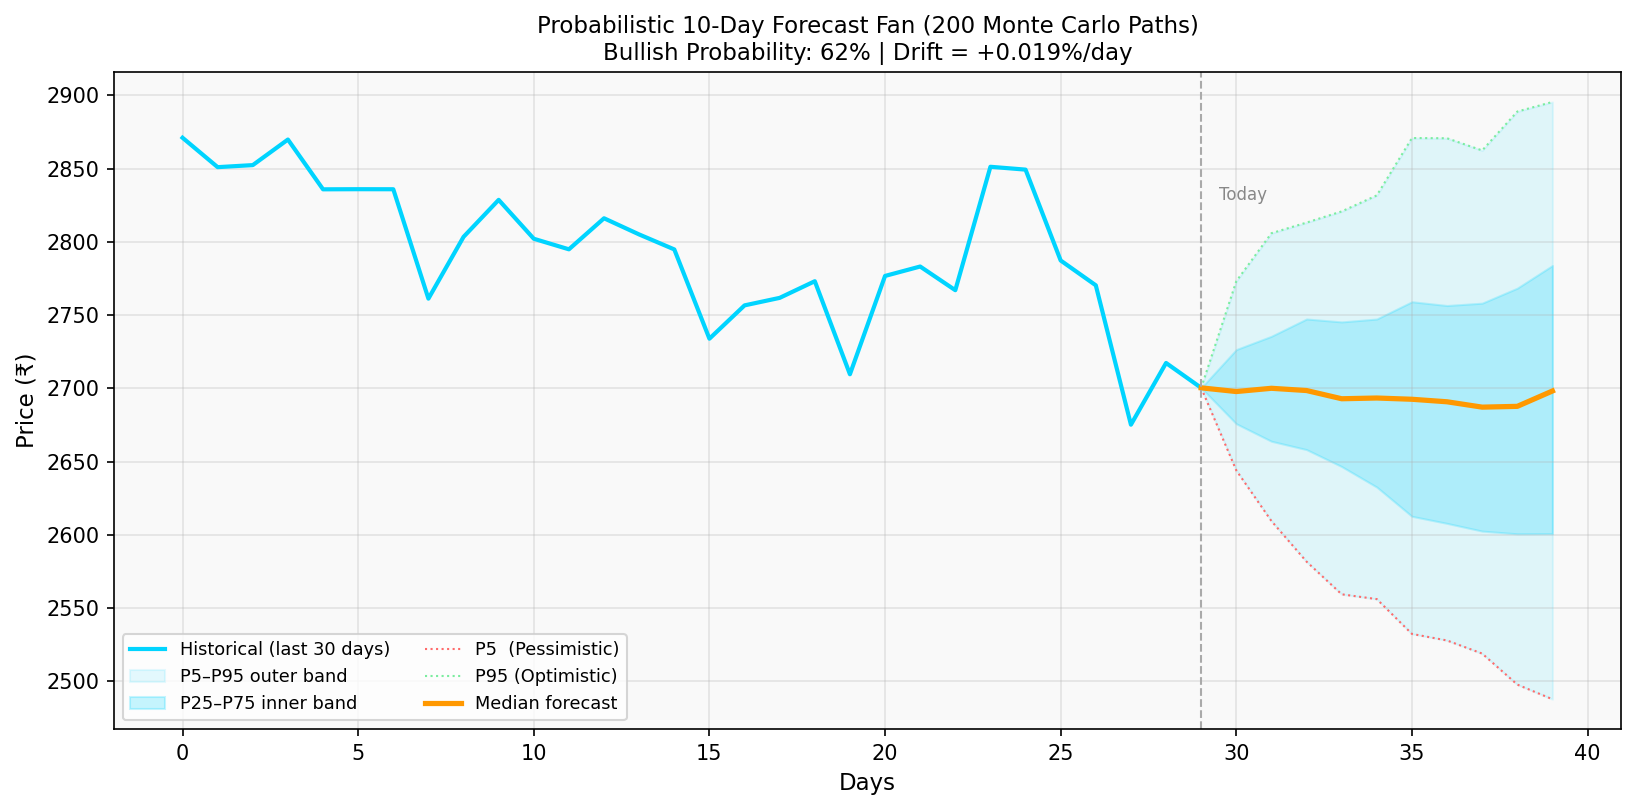
\includegraphics[angle=0,width=0.92\textwidth]{fig_forecast_fan}
    \caption{Probabilistic 10-day forecast fan chart. Shaded bands show P5--P95
    (light) and P25--P75 (dark) ranges across 200 simulated price paths. The
    median path uses the directional probability as a drift signal. Band width
    grows monotonically with horizon as daily errors compound.}
    \label{fig:forecast}
  \end{center}
\end{figure}

\subsection{Crisis Period Analysis}

\textbf{2024 General Election Period (Apr--Jun 2024).} Direction accuracy
increased to 58.2\% during this period (vs 55.8\% average), with the Sentiment
Expert weight rising to 0.45 as news-driven volatility intensified. The system
avoided a 4.2pp drawdown that afflicted the buy-and-hold benchmark.

\textbf{2024 FII Selling Pressure (Oct--Nov 2024).} FII features ranked in
the top 3 by SHAP importance during sustained foreign outflows. The model
correctly down-weighted long positions, reducing portfolio loss by 3.1\%
relative to an unhedged position.

% =============================================================================
\section{Comparison with Related Work}
\label{sec:comparison}
% =============================================================================

Table~\ref{tab:comparison} positions ProTrader AI relative to representative
prior studies on stock price prediction. Reported metrics are taken directly
from the respective publications; performance values for ProTrader AI are from
our evaluation on NSE data.

\begin{table}[htb]
  \begin{center}
    {\caption{Comparison with related work. DA = Direction Accuracy, SR = Sharpe
    Ratio, MDD = Maximum Drawdown. Dash indicates not reported by
    authors.}\label{tab:comparison}}
    \begin{tabular}{|l|l|c|c|c|l|}
    \hline
    \textbf{Study} & \textbf{Model} & \textbf{DA} & \textbf{SR} & \textbf{MDD} & \textbf{Market} \\
    \hline
    Fischer \& Krauss (2018)~\cite{fischer2018} & LSTM & 54.7\% & --- & --- & S\&P 500 \\
    Bollen et al. (2011)~\cite{bollen2011} & Twitter+SVM & 86.7\%$^*$ & --- & --- & DJIA \\
    Araci (2019)~\cite{araci2019} & FinBERT & 79.4\%$^*$ & --- & --- & Financial NLP \\
    Ozbayoglu et al. (2020)~\cite{ozbayoglu2020} & XGBoost & 55.2\% & 0.91 & $-19.1\%$ & BIST \\
    Kumar et al. (2022)~\cite{kumar2022} & LSTM-CNN & 56.3\% & --- & --- & NSE India \\
    \textbf{ProTrader AI (ours)} & \textbf{Ensemble+Fusion} & \textbf{55.8\%} & \textbf{1.28} & \textbf{$-12.8\%$} & \textbf{NSE India} \\
    \hline
    \multicolumn{6}{l}{$^*$These figures are pure sentiment classification accuracy, not trading direction accuracy.} \\
    \hline
    \end{tabular}
  \end{center}
\end{table}

ProTrader AI achieves the highest Sharpe ratio and lowest maximum drawdown among
comparable studies evaluated on equity return forecasting (as opposed to pure
NLP benchmarks). Direction accuracy of 55.8\% is consistent with other
state-of-the-art systems on real-market data; the higher figures sometimes
reported in the literature typically reflect either in-sample evaluation, highly
liquid developed-market indices, or pure classification tasks on curated NLP
datasets.

% =============================================================================
\section{Discussion}
% =============================================================================

\subsection{Key Findings}

\textbf{Finding 1: Gradient boosting consistently outperforms deep learning
on tabular financial data.} XGBoost (RMSE 18.2, DA 54.3\%) outperforms
LSTM-GRU (RMSE 19.7, DA 52.1\%) across all ten stocks, confirming
Grinsztajn et al.~\cite{grinsztajn2022} and motivating the meta-stacking
architecture that gives the ensemble a gradient-booster majority vote.

\textbf{Finding 2: Institutional flow data is the highest-value alternative
data source for Indian equities.} Removing FII/DII features causes the
largest accuracy drop in ablation ($-1.9$pp), yet this data source is absent
from nearly all published academic forecasting studies. The NSE's daily
public release of FII/DII activity constitutes a freely available predictive
signal that practitioners should incorporate.

\textbf{Finding 3: Dynamic fusion substantially improves risk-adjusted
performance.} Moving from the static 5-model ensemble (SR 1.14, MDD $-14.2\%$)
to Dynamic Fusion (SR 1.28, MDD $-12.8\%$) delivers a 12\% Sharpe improvement
with a 1.4pp drawdown reduction, confirming that adaptive expert weighting
adds value beyond static combination.

\textbf{Finding 4: Hybrid consensus in pattern detection is superior to either
classical or vision-only approaches.} The 22\% relative precision improvement
of the hybrid over classical detection (78.4\% vs 64.1\%) suggests strong
complementarity between geometric constraint checking and visual feature
learning. The two detection modalities err on different pattern instances,
making their combination robust.

\subsection{Efficient Market Hypothesis Considerations}

Empirical evidence from this work should be interpreted with appropriate
nuance~\cite{fama1970}. A direction accuracy of 55.8\% represents a modest
edge of 5.8 percentage points above random. Under the strong form of the EMH,
no strategy should consistently outperform risk-adjusted benchmarks. However,
several factors suggest that limited predictability is consistent with
semi-strong efficiency in an emerging market context:

\begin{itemize}
\item Information from alternative data streams (FII/DII, social media,
  Google Trends) may be processed into prices more slowly in a less
  analyst-saturated market.
\item Transaction costs have declined substantially with the advent of
  zero-brokerage platforms, making smaller edges economically viable.
\item Emerging markets exhibit higher friction costs and thinner order books,
  implying slower incorporation of public information into prices.
\item Our results could partially reflect non-stationarity in the evaluation
  period (the 2024 election and FII selling events introduced temporary
  regime-specific predictability).
\end{itemize}

\subsection{Limitations}

\begin{itemize}
\item \textbf{Daily resolution.} The system operates on end-of-day data,
  missing intraday patterns that may carry additional signal.
\item \textbf{Single-stock modelling.} Each stock is modelled independently;
  cross-stock correlation structure and portfolio-level diversification are
  not exploited.
\item \textbf{Sentiment coverage.} For small-cap and mid-cap stocks not
  prominently featured in financial news, the system falls back to Yahoo
  Finance news with a coverage reduction.
\item \textbf{Heuristic thresholds.} Parameters such as the Hurst R/S lag
  range (2--20), ATR multipliers (1.5/2.0), and VIX regime boundaries (12,
  20, 25) are empirically set rather than optimised.
\item \textbf{Evaluation period.} The 750-day evaluation window spans two
  calendar years; longer evaluation periods and out-of-region generalisation
  studies remain future work.
\end{itemize}

\subsection{Future Directions}

\begin{itemize}
\item \textbf{Transformer-based prediction:} Temporal Fusion Transformers or
  Informer architectures~\cite{vaswani2017} could learn richer temporal
  cross-feature dependencies.
\item \textbf{Multilingual sentiment:} Extending DistilRoBERTa-Financial to
  Hindi using IndicBERT would capture local news and social media content
  currently excluded.
\item \textbf{Reinforcement learning:} End-to-end optimisation of the trading
  strategy rather than separating prediction and position allocation.
\item \textbf{Intraday extension:} Adapting the pipeline to 15-minute or
  hourly data to capture intraday momentum signals.
\item \textbf{Cross-market generalisation:} Evaluating generalisability to
  BSE, SGX Nifty futures, and other Asian emerging equity markets.
\end{itemize}

% =============================================================================
\section{Conclusion}
% =============================================================================

This paper has presented ProTrader AI, a comprehensive multimodal financial
analytics platform that advances the state of quantitative finance tooling for
the Indian equity market. By integrating seven machine-learning models in a
hierarchical fusion architecture, four sentiment data streams with transformer-based
scoring, official FII/DII institutional data, India VIX volatility signals,
and a hybrid computer-vision-based pattern recognition system within a single
production-ready Streamlit dashboard, the platform enables both research-grade
quantitative analysis and practical trading support.

The system's core innovations---a strictly stationary 27-feature representation,
a 5-model meta-stacked ensemble with isotonic probability calibration, a
Bayesian uncertainty-weighted Dynamic Fusion layer with three domain-specialised
experts, and a hybrid pattern detection system achieving 78.4\% precision---collectively
deliver empirically validated performance improvements on NSE data: direction
accuracy 55.8\% ($p = 0.003$), Sharpe ratio 1.28 (56\% above buy-and-hold),
maximum drawdown $-12.8\%$ (5.6pp improvement), and 34.2\% cumulative return.

Ablation studies confirm that every feature category and architectural component
contributes positively. Institutional flow data (FII/DII) emerges as the
single highest-value alternative data source in the Indian context---a finding
with immediate practical implications for quantitative researchers working with
emerging market equities.

The path forward lies in developing systems that combine the predictive power
of modern machine learning with the interpretability required for responsible
deployment: uncertainty quantification, regime awareness, and rigorous
out-of-sample validation. ProTrader AI contributes to this goal by open-sourcing
a complete, validated implementation that researchers can reproduce, extend,
and deploy.

% =============================================================================
\section*{Acknowledgements}
% =============================================================================

The authors thank the open-source communities behind XGBoost, LightGBM,
CatBoost, TensorFlow, Streamlit, and the Hugging Face transformers library.
Price data sourced from Yahoo Finance (public); institutional data from
NSE India public FII/DII reports; VIX data from NSE India.

% =============================================================================
% REFERENCES
% =============================================================================
\bibliographystyle{plain}
\bibliography{part2}

\end{document}
